\subsection{In Sample Regressions}
\begin{table}
	\centering \caption{\textbf{:Full In Sample Results} \newline
		\footnotesize{The table displays in sample regression results for monthly market variance, correlation and return statistics. SV is the annualized monthly variance of daily CRSP market returns. AV and AC are the monthly average variance and average pairwise correlation of daily returns for the top 500 assets in the CRSP market, as in \citet{pollet_average_2010}. RET is the log return of the CRSP market portfolio minus the log return on the 1 month treasury bill. The sample period is from 1926:07 to 2016:12. The coefficients and p-values are robust, see section \ref{sec:in_sample} for details.}} \vspace{-3mm}
	\label{tab:tab_in_sample_full_app}
	\subcaption{Market Return Variance - SV$_{t+1}$}\vspace{-3mm}
	\begin{adjustbox}{center,max height=.45\totalheight}
		
% Table created by stargazer v.5.2 by Marek Hlavac, Harvard University. E-mail: hlavac at fas.harvard.edu
% Date and time: Fri, Jun 08, 2018 - 12:52:08  IST
\begin{tabular}{@{\extracolsep{5pt}}lccccc} 
\\[-1.8ex]
\hline \\[-1.8ex] 
AV & 0.627$^{***}$ &  &  & 0.553$^{***}$ & 0.368$^{***}$ \\ 
& p = 0.000 &  &  & p = 0.000 & p = 0.000 \\ 
%& & & & & \\ 
AC &  & 0.418$^{***}$ &  & 0.160$^{***}$ &  \\ 
&  & p = 0.000 &  & p = 0.000 &  \\ 
%& & & & & \\ 
SV &  &  & 0.615$^{***}$ &  & 0.278$^{***}$ \\ 
&  &  & p = 0.000 &  & p = 0.000 \\ 
%& & & & & \\ 
Constant & $-$0.0003 & $-$0.0001 & $-$0.0002 & $-$0.0003 & $-$0.0003 \\ 
& p = 0.991 & p = 0.998 & p = 0.993 & p = 0.991 & p = 0.991 \\ 
%& & & & & \\ 
%\textit{N} & 1,085 & 1,085 & 1,085 & 1,085 & 1,085 \\ 
R$^{2}$ & 0.391 & 0.173 & 0.375 & 0.410 & 0.413 \\ 
Adjusted R$^{2}$ & 0.390 & 0.173 & 0.374 & 0.409 & 0.412 \\ 
%\hline 
\hline \\[-1.8ex] 
%\textit{Notes:} & \multicolumn{5}{r}{$^{***}$Significant at the 1 percent level.} \\ 
% & \multicolumn{5}{r}{$^{**}$Significant at the 5 percent level.} \\ 
% & \multicolumn{5}{r}{$^{*}$Significant at the 10 percent level.} \\ 
\end{tabular} 

	\end{adjustbox}
	\subcaption{Average Asset Return Variance - AV$_{t+1}$}\vspace{-3mm}
	\begin{adjustbox}{center,max height=.45\totalheight}
		
% Table created by stargazer v.5.2 by Marek Hlavac, Harvard University. E-mail: hlavac at fas.harvard.edu
% Date and time: Thu, Apr 05, 2018 - 02:23:32  IST
\begin{tabular}{@{\extracolsep{5pt}}lccccc} 
%\\[-1.8ex]\hline 
%\hline \\[-1.8ex] 
%\\[-1.8ex] & \multicolumn{5}{c}{AV$_{t+1}$} \\ 
\hline \\[-1.8ex] 
 AV & 0.718$^{***}$ &  &  & 0.705$^{***}$ & 0.745$^{***}$ \\ 
%  & p = 0.000 &  &  & p = 0.000 & p = 0.000 \\ 
  & & & & & \\ 
 AC &  & 0.034$^{***}$ &  & 0.003 &  \\ 
%  &  & p = 0.000 &  & p = 0.232 &  \\ 
  & & & & & \\ 
 SV &  &  & 1.549$^{***}$ &  & $-$0.080 \\ 
%  &  &  & p = 0.000 &  & p = 0.445 \\ 
  & & & & & \\ 
 Constant & 0.002$^{***}$ & $-$0.001 & 0.005$^{***}$ & 0.002$^{***}$ & 0.002$^{***}$ \\ 
%  & p = 0.000 & p = 0.463 & p = 0.000 & p = 0.004 & p = 0.000 \\ 
  & & & & & \\ 
%\textit{N} & 1,085 & 1,085 & 1,085 & 1,085 & 1,085 \\ 
R$^{2}$ & 0.515 & 0.128 & 0.368 & 0.516 & 0.516 \\ 
Adjusted R$^{2}$ & 0.515 & 0.127 & 0.367 & 0.515 & 0.515 \\ 
\hline 
%\hline \\[-1.8ex] 
%\textit{Notes:} & \multicolumn{5}{r}{$^{***}$Significant at the 1 percent level.} \\ 
% & \multicolumn{5}{r}{$^{**}$Significant at the 5 percent level.} \\ 
% & \multicolumn{5}{r}{$^{*}$Significant at the 10 percent level.} \\ 
\end{tabular} 

	\end{adjustbox}
	\subcaption{Average Asset Return Correlation - AC$_{t+1}$}\vspace{-3mm}
	\begin{adjustbox}{center,max height=.45\totalheight}
		
% Table created by stargazer v.5.2 by Marek Hlavac, Harvard University. E-mail: hlavac at fas.harvard.edu
% Date and time: Fri, Jun 08, 2018 - 12:50:47  IST
\begin{tabular}{@{\extracolsep{5pt}}lccccc} 
%\\[-1.8ex]\hline 
%\hline \\[-1.8ex] 
%\\[-1.8ex] & \multicolumn{5}{c}{AC$_{t+1}$} \\ 
\\[-1.8ex]
\hline \\[-1.8ex] 
 AV & 0.384$^{***}$ &  &  & 0.125$^{***}$ & $-$0.029 \\ 
  & p = 0.000 &  &  & p = 0.00001 & p = 0.641 \\ 
%  & & & & & \\ 
 AC &  & 0.613$^{***}$ &  & 0.554$^{***}$ &  \\ 
  &  & p = 0.000 &  & p = 0.000 &  \\ 
%  & & & & & \\ 
 SV &  &  & 0.454$^{***}$ &  & 0.458$^{***}$ \\ 
  &  &  & p = 0.000 &  & p = 0.000 \\ 
%  & & & & & \\ 
 Constant & $-$0.0002 & $-$0.0001 & $-$0.0002 & $-$0.0002 & $-$0.0002 \\ 
  & p = 0.996 & p = 0.996 & p = 0.996 & p = 0.995 & p = 0.996 \\ 
%  & & & & & \\ 
%\textit{N} & 1,085 & 1,085 & 1,085 & 1,085 & 1,085 \\ 
R$^{2}$ & 0.147 & 0.372 & 0.205 & 0.385 & 0.205 \\ 
Adjusted R$^{2}$ & 0.146 & 0.372 & 0.204 & 0.384 & 0.204 \\ 
%\hline 
\hline \\[-1.8ex] 
%\textit{Notes:} & \multicolumn{5}{r}{$^{***}$Significant at the 1 percent level.} \\ 
% & \multicolumn{5}{r}{$^{**}$Significant at the 5 percent level.} \\ 
% & \multicolumn{5}{r}{$^{*}$Significant at the 10 percent level.} \\ 
\end{tabular} 

	\end{adjustbox}
	\subcaption{Log Excess Market Return - RET$_{t+1}$}\vspace{-3mm}
	\begin{adjustbox}{center,max height=.45\totalheight}
		% Table created by stargazer v.5.2 by Marek Hlavac, Harvard University. E-mail: hlavac at fas.harvard.edu
% Date and time: Fri, Jun 08, 2018 - 12:54:38  IST
\begin{tabular}{@{\extracolsep{5pt}}lccccc} 
%\\[-1.8ex]\hline 
\hline \\[-1.8ex] 
% & \multicolumn{5}{c}{RET$_{t+1}$ - 1926M7:2016M12} \\ 
%\\[-1.8ex]
\hline \\[-1.8ex] 
 AV & -0.0002 &  &  & $-$0.006 & 0.192 \\ 
  & p = 0.562 &  &  & p = $0.423$ & p = $0.833$ \\ 
%  & & & & & \\ 
 AC &  & 0.010$^{**}$ &  & 0.012$^{**}$ &  \\ 
  &  & p = 0.0.052 &  & p = $0.068$ &  \\ 
%  & & & & & \\ 
 SV &  &  & $-$0.057 &  & $-$0.204 \\ 
  &  &  & p = $0.612$ &  & p = $0.865$ \\ 
%  & & & & & \\ 
% Constant & $-$0.00000 & $-$0.00001 & 0.00002 & $-$0.00001 & 0.00002 \\ 
%  & p = 1.000 & p = 1.000 & p = 1.000 & p = 1.000 & p = 1.000 \\ 
%  & & & & & \\ 
%\textit{N} & 1,085 & 1,085 & 1,085 & 1,085 & 1,085 \\ 
R$^{2}$ & 0.00000 & 0.0001 & 0.003 & 0.0001 & 0.012 \\ 
Adjusted R$^{2}$ & $-$0.001 & $-$0.001 & 0.002 & $-$0.002 & 0.010 \\ 
%\hline 
\hline \\[-1.8ex] 
%\textit{Notes:} & \multicolumn{5}{r}{$^{***}$,$^{**}$, and $^{*}$ Significant at the 1, 5, and 10 percent levels.} \\ 
% & \multicolumn{5}{r}{$^{**}$Significant at the 5 percent level.} \\ 
% & \multicolumn{5}{r}{$^{*}$Significant at the 10 percent level.} \\ 
\end{tabular} 
	\end{adjustbox}
\end{table}
\clearpage
\begin{table}[!htbp]
	\centering \caption{\textbf{:In Sample Results - Pre 1962} \newline
		\footnotesize{The table displays in sample regression results for monthly market variance, correlation and return statistics. SV is the annualized monthly variance of daily CRSP market returns. AV and AC are the monthly average variance and average pairwise correlation of daily returns for the top 500 assets in the CRSP market, as in \citet{pollet_average_2010}. RET is the log return of the CRSP market portfolio minus the log return on the 1 month treasury bill. The sample period is from 1926:07 to 2016:1962:06. The series are standardized to a mean of zero and standard deviation of one. The coefficients and p-values are robust, see section \ref{sec:in_sample} for details.}} \vspace{-3mm}
	\label{tab:tab_in_sample_1962}
	\subcaption{Market Return Variance - SV$_{t+1}$}\vspace{-3mm}
	\begin{adjustbox}{center,max height=.45\totalheight}
		
% Table created by stargazer v.5.2 by Marek Hlavac, Harvard University. E-mail: hlavac at fas.harvard.edu
% Date and time: Fri, Jun 08, 2018 - 12:56:59  IST
\begin{tabular}{@{\extracolsep{5pt}}lccccc} 
%\\[-1.8ex]\hline 
%\hline \\[-1.8ex] 
%& \multicolumn{5}{c}{SV$_{t+1}$} 
\\ 
\hline \\[-1.8ex] 
 AV & 0.672$^{***}$ &  &  & 0.583$^{***}$ & 0.414$^{***}$ \\ 
  & p = 0.000 &  &  & p = 0.000 & p = 0.000 \\ 
%  & & & & & \\ 
 AC &  & 0.492$^{***}$ &  & 0.160$^{***}$ &  \\ 
  &  & p = 0.000 &  & p = 0.0004 &  \\ 
%  & & & & & \\ 
 SV &  &  & 0.650$^{***}$ &  & 0.266$^{***}$ \\ 
  &  &  & p = 0.000 &  & p = 0.00004 \\ 
%  & & & & & \\ 
 Constant & $-$0.000 & $-$0.000 & 0.000 & $-$0.000 & 0.000 \\ 
  & p = 1.000 & p = 1.000 & p = 1.000 & p = 1.000 & p = 1.000 \\ 
%  & & & & & \\ 
%\textit{N} & 432 & 432 & 432 & 432 & 432 \\ 
R$^{2}$ & 0.444 & 0.236 & 0.413 & 0.460 & 0.466 \\ 
Adjusted R$^{2}$ & 0.443 & 0.235 & 0.412 & 0.458 & 0.463 \\ 
%\hline 
\hline \\[-1.8ex] 
%\textit{Notes:} & \multicolumn{5}{r}{$^{***}$Significant at the 1 percent level.} \\ 
% & \multicolumn{5}{r}{$^{**}$Significant at the 5 percent level.} \\ 
% & \multicolumn{5}{r}{$^{*}$Significant at the 10 percent level.} \\ 
\end{tabular} 

%\begin{tabular}{@{\extracolsep{5pt}} cccccccccccccc} 
%	\\[-1.8ex]\hline 
%	\hline \\[-1.8ex] 
%	& Y & Form & avg\_var1m & t.stat.avg\_var1m & p.val.avg\_var1m & avg\_cor1m & t.stat.avg\_cor1m & p.val.avg\_cor1m & mkt\_var1m & t.stat.mkt\_var1m & p.val.mkt\_var1m & r.squared & adj.r.squared \\ 
%	\hline \\[-1.8ex] 
%	1 & mkt\_var1m.tp1 & mkt\_var1m.tp1 \textasciitilde avg\_var1m & $0.672$ & $26.293$ & $0$ & $$ & $$ & $$ & $$ & $$ & $$ & $0.720$ & $0.719$ \\ 
%	2 & mkt\_var1m.tp1 & mkt\_var1m.tp1 \textasciitilde avg\_cor1m & $$ & $$ & $$ & $0.492$ & $14.550$ & $0$ & $$ & $$ & $$ & $0.514$ & $0.512$ \\ 
%	3 & mkt\_var1m.tp1 & mkt\_var1m.tp1 \textasciitilde mkt\_var1m & $$ & $$ & $$ & $$ & $$ & $$ & $0.650$ & $54,021,381,181,960,992$ & $0$ & $1$ & $1$ \\ 
%	4 & mkt\_var1m.tp1 & mkt\_var1m.tp1 \textasciitilde avg\_var1m + avg\_cor1m & $0.583$ & $21.588$ & $0$ & $0.160$ & $5.926$ & $0$ & $$ & $$ & $$ & $0.792$ & $0.791$ \\ 
%	5 & mkt\_var1m.tp1 & mkt\_var1m.tp1 \textasciitilde avg\_var1m + mkt\_var1m & $0.414$ & $23,526,287,727,722,408$ & $0$ & $$ & $$ & $$ & $0.266$ & $15,091,978,274,695,688$ & $0$ & $1$ & $1$ \\ 
%	\hline \\[-1.8ex] 
%\end{tabular} 


	\end{adjustbox}
	\subcaption{Average Asset Return Variance - AV$_{t+1}$}\vspace{-3mm}
	\begin{adjustbox}{center,max height=.45\totalheight}
		
% Table created by stargazer v.5.2 by Marek Hlavac, Harvard University. E-mail: hlavac at fas.harvard.edu
% Date and time: Thu, Apr 05, 2018 - 02:28:21  IST
\begin{tabular}{@{\extracolsep{5pt}}lccccc} 
\\[-1.8ex]\hline 
\hline \\[-1.8ex] 
\\[-1.8ex] & \multicolumn{5}{c}{AV$_{t+1}$} \\ 
\hline \\[-1.8ex] 
 AV & 0.732$^{***}$ &  &  & 0.691$^{***}$ & 0.641$^{***}$ \\ 
  & p = 0.000 &  &  & p = 0.000 & p = 0.000 \\ 
  & & & & & \\ 
 AC &  & 0.058$^{***}$ &  & 0.009$^{*}$ &  \\ 
  &  & p = 0.000 &  & p = 0.080 &  \\ 
  & & & & & \\ 
 SV &  &  & 1.833$^{***}$ &  & 0.301$^{*}$ \\ 
  &  &  & p = 0.000 &  & p = 0.084 \\ 
  & & & & & \\ 
 Constant & 0.003$^{***}$ & $-$0.007$^{***}$ & 0.005$^{***}$ & 0.001 & 0.003$^{***}$ \\ 
  & p = 0.00003 & p = 0.0001 & p = 0.000 & p = 0.667 & p = 0.00003 \\ 
  & & & & & \\ 
\textit{N} & 432 & 432 & 432 & 432 & 432 \\ 
R$^{2}$ & 0.535 & 0.218 & 0.422 & 0.539 & 0.539 \\ 
Adjusted R$^{2}$ & 0.534 & 0.216 & 0.420 & 0.537 & 0.537 \\ 
\hline 
\hline \\[-1.8ex] 
\textit{Notes:} & \multicolumn{5}{r}{$^{***}$Significant at the 1 percent level.} \\ 
 & \multicolumn{5}{r}{$^{**}$Significant at the 5 percent level.} \\ 
 & \multicolumn{5}{r}{$^{*}$Significant at the 10 percent level.} \\ 
\end{tabular} 

	\end{adjustbox}
	\subcaption{Average Asset Return Correlation - AC$_{t+1}$}\vspace{-3mm}
	\begin{adjustbox}{center,max height=.45\totalheight}
		
% Table created by stargazer v.5.2 by Marek Hlavac, Harvard University. E-mail: hlavac at fas.harvard.edu
% Date and time: Thu, Apr 05, 2018 - 02:26:04  IST
\begin{tabular}{@{\extracolsep{5pt}}lccccc} 
\\[-1.8ex]\hline 
\hline \\[-1.8ex] 
\\[-1.8ex] & \multicolumn{5}{c}{AC$_{t+1}$} \\ 
\hline \\[-1.8ex] 
 AV & 3.992$^{***}$ &  &  & 2.019$^{***}$ & 1.316$^{**}$ \\ 
  & p = 0.000 &  &  & p = 0.00000 & p = 0.031 \\ 
  & & & & & \\ 
 AC &  & 0.575$^{***}$ &  & 0.430$^{***}$ &  \\ 
  &  & p = 0.000 &  & p = 0.000 &  \\ 
  & & & & & \\ 
 SV &  &  & 12.069$^{***}$ &  & 8.927$^{***}$ \\ 
  &  &  & p = 0.000 &  & p = 0.00000 \\ 
  & & & & & \\ 
 Constant & 0.258$^{***}$ & 0.128$^{***}$ & 0.261$^{***}$ & 0.150$^{***}$ & 0.257$^{***}$ \\ 
  & p = 0.000 & p = 0.000 & p = 0.000 & p = 0.000 & p = 0.000 \\ 
  & & & & & \\ 
\textit{N} & 432 & 432 & 432 & 432 & 432 \\ 
R$^{2}$ & 0.249 & 0.331 & 0.286 & 0.374 & 0.294 \\ 
Adjusted R$^{2}$ & 0.248 & 0.329 & 0.285 & 0.371 & 0.291 \\ 
\hline 
\hline \\[-1.8ex] 
\textit{Notes:} & \multicolumn{5}{r}{$^{***}$Significant at the 1 percent level.} \\ 
 & \multicolumn{5}{r}{$^{**}$Significant at the 5 percent level.} \\ 
 & \multicolumn{5}{r}{$^{*}$Significant at the 10 percent level.} \\ 
\end{tabular} 

	\end{adjustbox}
	\subcaption{Log Excess Market Return - RET$_{t+1}$}\vspace{-3mm}
	\begin{adjustbox}{center,max height=.45\totalheight}
		
% Table created by stargazer v.5.2 by Marek Hlavac, Harvard University. E-mail: hlavac at fas.harvard.edu
% Date and time: Fri, Jun 08, 2018 - 12:59:10  IST
\begin{tabular}{@{\extracolsep{5pt}}lccccc} 
%\\[-1.8ex]\hline 
%\hline \\[-1.8ex] 
%& \multicolumn{5}{c}{RET$_{t+1}$ - 1926M7:1962M6} \\
\hline \\[-1.8ex] 
 AV & $0.061$ &  &  & $0.121$ & $0.315$ \\ 
  & p = $0.609$ &  &  & p = $0.741$ & p = $0.954$ \\ 
%  & & & & & \\ 
 AC &  & $-$0.032 &  & $-$0.099 &  \\ 
  &  & p = 0.520 &  & p = $0.862$ &  \\ 
%  & & & & & \\ 
 SV &  &  & $-$0.028 &  & $-$0.264 \\ 
  &  &  & p = 0.418 &  & p = $0.948$ \\ 
%  & & & & & \\ 
% Constant & $-$0.0001 & 0.0001 & 0.00003 & 0.0001 & 0.00004 \\ 
%  & p = 1.000 & p = 1.000 & p = 1.000 & p = 0.999 & p = 1.000 \\ 
%  & & & & & \\ 
%\textit{N} & 431 & 431 & 431 & 431 & 431 \\ 
R$^{2}$ & 0.004 & 0.001 & 0.001 & 0.010 & 0.026 \\ 
Adjusted R$^{2}$ & 0.002 & $-$0.002 & $-$0.002 & 0.005 & 0.021 \\ 
%\hline 
\hline \\[-1.8ex] 
%\textit{Notes:} & \multicolumn{5}{r}{$^{***}$,$^{**}$, and $^{*}$ Significant at the 1, 5, and 10 percent levels.} \\  
\end{tabular} 

%\begin{tabular}{@{\extracolsep{5pt}} cccccccccccccc} 
%	\\[-1.8ex]\hline 
%	\hline \\[-1.8ex] 
%	& Y & Form & avg\_var1m & t.stat.avg\_var1m & p.val.avg\_var1m & avg\_cor1m & t.stat.avg\_cor1m & p.val.avg\_cor1m & mkt\_var1m & t.stat.mkt\_var1m & p.val.mkt\_var1m & r.squared & adj.r.squared \\ 
%	\hline \\[-1.8ex] 
%	1 & logxret.tp1 & logxret.tp1 \textasciitilde avg\_var1m & $0.061$ & $1.292$ & $0.609$ & $$ & $$ & $$ & $$ & $$ & $$ & $0.032$ & $0.028$ \\ 
%	2 & logxret.tp1 & logxret.tp1 \textasciitilde avg\_cor1m & $$ & $$ & $$ & $$-$0.032$ & $$-$0.718$ & $0.520$ & $$ & $$ & $$ & $0.183$ & $0.179$ \\ 
%	3 & logxret.tp1 & logxret.tp1 \textasciitilde mkt\_var1m & $$ & $$ & $$ & $$ & $$ & $$ & $$-$0.028$ & $$-$0.601$ & $0.582$ & $0.083$ & $0.079$ \\ 
%	4 & logxret.tp1 & logxret.tp1 \textasciitilde avg\_var1m + avg\_cor1m & $0.121$ & $2.331$ & $0.741$ & $$-$0.099$ & $$-$1.898$ & $0.862$ & $$ & $$ & $$ & $0.228$ & $0.221$ \\ 
%	5 & logxret.tp1 & logxret.tp1 \textasciitilde avg\_var1m + mkt\_var1m & $0.315$ & $3.796$ & $0.954$ & $$ & $$ & $$ & $$-$0.264$ & $$-$3.178$ & $0.948$ & $0.166$ & $0.158$ \\ 
%	\hline \\[-1.8ex] 
%\end{tabular} 
	\end{adjustbox}
\end{table}
\clearpage
\begin{table}[!htbp]
	\centering \caption{\textbf{:In Sample Results - Post 1962} \newline
		\footnotesize{The table displays in sample regression results for monthly market variance, correlation and return statistics. SV is the annualized monthly variance of daily CRSP market returns. AV and AC are the monthly average variance and average pairwise correlation of daily returns for the top 500 assets in the CRSP market, as in \citet{pollet_average_2010}. RET is the log return of the CRSP market portfolio minus the log return on the 1 month treasury bill. The sample period is from 1962:06 to 2016:12. The series are standardized to a mean of zero and standard deviation of one. The coefficients and p-values are robust, see section \ref{sec:in_sample} for details.}} \vspace{-3mm}
	\label{tab:tab_in_sample_2016}
	\subcaption{Market Return Variance - SV$_{t+1}$}\vspace{-3mm}
	\begin{adjustbox}{center,max height=.45\totalheight}
		
% Table created by stargazer v.5.2 by Marek Hlavac, Harvard University. E-mail: hlavac at fas.harvard.edu
% Date and time: Fri, Jun 08, 2018 - 01:01:25  IST
\begin{tabular}{@{\extracolsep{5pt}}lccccc} 
\\
\hline \\[-1.8ex] 
%\\[-1.8ex] & \multicolumn{5}{c}{SV$_{t+1}$} \\ 
%\\[-1.8ex] 
\hline \\[-1.8ex] 
 AV & 0.550$^{***}$ &  &  & 0.494$^{***}$ & 0.135$^{***}$ \\ 
  & p = 0.000 &  &  & p = 0.000 & p = 0.001 \\ 
% & & & & & \\ 
 AC &  & 0.334$^{***}$ &  & 0.162$^{***}$ &  \\ 
  &  & p = 0.000 &  & p = 0.00001 &  \\ 
%  & & & & & \\ 
 SV &  &  & 0.556$^{***}$ &  & 0.187$^{***}$ \\ 
  &  &  & p = 0.000 &  & p = 0.00002 \\ 
% & & & & & \\ 
 Constant & $-$0.0005 & $-$0.0001 & $-$0.0003 & $-$0.0005 & $-$0.0004 \\ 
  & p = 0.989 & p = 0.999 & p = 0.993 & p = 0.989 & p = 0.991 \\ 
%  & & & & & \\ 
%\textit{N} & 654 & 654 & 654 & 654 & 654 \\ 
R$^{2}$ & 0.297 & 0.110 & 0.304 & 0.320 & 0.317 \\ 
Adjusted R$^{2}$ & 0.296 & 0.109 & 0.303 & 0.318 & 0.315 \\ 
\hline \\[-1.8ex] 
%\textit{Notes:} & \multicolumn{5}{r}{$^{***}$Significant at the 1 percent level.} \\ 
% & \multicolumn{5}{r}{$^{**}$Significant at the 5 percent level.} \\ 
% & \multicolumn{5}{r}{$^{*}$Significant at the 10 percent level.} \\ 
\end{tabular} 

%\begin{tabular}{@{\extracolsep{5pt}}lccccc} 
%	\\[-1.8ex]\hline 
%	\hline \\[-1.8ex] 
%	\\[-1.8ex] & \multicolumn{5}{c}{SV$_{t+1}$} \\ 
%	\hline \\[-1.8ex] 
% AV & 0.545$^{***}$ &  &  & 0.489$^{***}$ & 0.257$^{***}$ \\ 
% & p = 0.000 &  &  & p = 0.000 & p = 0.001 \\ 
%   & & & & & \\ 
% AC &  & 0.332$^{***}$ &  & 0.160$^{***}$ &  \\ 
% &  & p = 0.000 &  & p = 0.00001 &  \\ 
%   & & & & & \\ 
% SV &  &  & 0.551$^{***}$ &  & 0.320$^{***}$ \\ 
% &  &  & p = 0.000 &  & p = 0.00002 \\ 
%  & & & & & \\ 
% Constant & $-$0.0005 & $-$0.0001 & $-$0.0003 & $-$0.0005 & $-$0.0004 \\ 
% & p = 0.989 & p = 0.999 & p = 0.993 & p = 0.989 & p = 0.991 \\ 
%   & & & & & \\ 
% \textit{N} & 654 & 654 & 654 & 654 & 654 \\ 
% R$^{2}$ & 0.297 & 0.110 & 0.304 & 0.320 & 0.317 \\ 
% Adjusted R$^{2}$ & 0.296 & 0.109 & 0.303 & 0.318 & 0.315 \\ 
% \hline \\[-1.8ex] 
%	\hline \\[-1.8ex] 
%	\textit{Notes:} & \multicolumn{5}{r}{$^{***}$Significant at the 1 percent level.} \\ 
%	& \multicolumn{5}{r}{$^{**}$Significant at the 5 percent level.} \\ 
%	& \multicolumn{5}{r}{$^{*}$Significant at the 10 percent level.} \\ 

	\end{adjustbox}
	\subcaption{Average Asset Return Variance - AV$_{t+1}$}\vspace{-3mm}
	\begin{adjustbox}{center,max height=.45\totalheight}
		
% Table created by stargazer v.5.2 by Marek Hlavac, Harvard University. E-mail: hlavac at fas.harvard.edu
% Date and time: Fri, Jun 08, 2018 - 01:02:34  IST
\begin{tabular}{@{\extracolsep{5pt}}lccccc} 
\\[-1.8ex]\hline 
\hline \\[-1.8ex] 
\\[-1.8ex] & \multicolumn{5}{c}{AV$_{t+1}$} \\ 
\hline \\[-1.8ex] 
 AV & 0.667$^{***}$ &  &  & 0.674$^{***}$ & 1.030$^{***}$ \\ 
  & p = 0.000 &  &  & p = 0.000 & p = 0.000 \\ 
  & & & & & \\ 
 AC &  & 0.218$^{***}$ &  & $-$0.019 &  \\ 
  &  & p = 0.00000 &  & p = 0.544 &  \\ 
  & & & & & \\ 
 SV &  &  & 0.522$^{***}$ &  & $-$0.403$^{***}$ \\ 
  &  &  & p = 0.000 &  & p = 0.000 \\ 
  & & & & & \\ 
 Constant & $-$0.001 & $-$0.00004 & $-$0.0003 & $-$0.001 & $-$0.001 \\ 
  & p = 0.985 & p = 1.000 & p = 0.994 & p = 0.984 & p = 0.981 \\ 
  & & & & & \\ 
\textit{N} & 654 & 654 & 654 & 654 & 654 \\ 
R$^{2}$ & 0.445 & 0.048 & 0.273 & 0.446 & 0.477 \\ 
Adjusted R$^{2}$ & 0.445 & 0.046 & 0.272 & 0.444 & 0.475 \\ 
\hline 
\hline \\[-1.8ex] 
\textit{Notes:} & \multicolumn{5}{r}{$^{***}$Significant at the 1 percent level.} \\ 
 & \multicolumn{5}{r}{$^{**}$Significant at the 5 percent level.} \\ 
 & \multicolumn{5}{r}{$^{*}$Significant at the 10 percent level.} \\ 
\end{tabular} 

	\end{adjustbox}
	\subcaption{Average Asset Return Correlation - AC$_{t+1}$}\vspace{-3mm}
	\begin{adjustbox}{center,max height=.45\totalheight}
		
% Table created by stargazer v.5.2 by Marek Hlavac, Harvard University. E-mail: hlavac at fas.harvard.edu
% Date and time: Fri, Jun 08, 2018 - 01:00:16  IST
\begin{tabular}{@{\extracolsep{5pt}}lccccc} 
%\\[-1.8ex]\hline 
%\hline \\[-1.8ex] 
%\\[-1.8ex] & \multicolumn{5}{c}{AC$_{t+1}$} \\
\\[-1.8ex]
\hline \\[-1.8ex] 
 AV & 0.241$^{***}$ &  &  & 0.023$^{***}$ & $-$0.634 \\ 
  & p = 0.000 &  &  & p = 0.000 & p = 0.999 \\ 
%  & & & & & \\ 
 AC &  & 0.626$^{***}$ &  & 0.619$^{***}$ &  \\ 
  &  & p = 0.000 &  & p = 0.000 &  \\ 
%  & & & & & \\ 
 SV &  &  & 0.362$^{***}$ &  & 0.539$^{***}$ \\ 
  &  &  & p = 0.000 &  & p = 0.008 \\ 
%  & & & & & \\ 
 Constant & $-$0.0002 & $-$0.0001 & $-$0.0002 & $-$0.0001 & $-$0.00003 \\ 
  & p = 0.996 & p = 0.998 & p = 0.996 & p = 0.997 & p = 1.000 \\ 
%  & & & & & \\ 
%\textit{N} & 654 & 654 & 654 & 654 & 654 \\ 
R$^{2}$ & 0.057 & 0.387 & 0.130 & 0.387 & 0.167 \\ 
Adjusted R$^{2}$ & 0.056 & 0.386 & 0.128 & 0.385 & 0.164 \\ 
%\hline 
\hline \\[-1.8ex] 
%\textit{Notes:} & \multicolumn{5}{r}{$^{***}$Significant at the 1 percent level.} \\ 
% & \multicolumn{5}{r}{$^{**}$Significant at the 5 percent level.} \\ 
% & \multicolumn{5}{r}{$^{*}$Significant at the 10 percent level.} \\ 
\end{tabular} 

	\end{adjustbox}
	\subcaption{Log Excess Market Return - RET$_{t+1}$}\vspace{-3mm}
	\begin{adjustbox}{center,max height=.45\totalheight}
		
% Table created by stargazer v.5.2 by Marek Hlavac, Harvard University. E-mail: hlavac at fas.harvard.edu
% Date and time: Fri, Jun 08, 2018 - 01:03:43  IST
\begin{tabular}{@{\extracolsep{5pt}}lccccc} 
%\\[-1.8ex]\hline 
%\hline \\[-1.8ex] 
%& \multicolumn{5}{c}{RET$_{t+1}$ - 1962M6:2016M12} \\ 
\\[-1.8ex]
\hline \\[-1.8ex] 
 AV & $-$0.131 &  &  & $-$0.168$^{**}$ & $0.016$ \\ 
  & p = 0.161 &  &  & p = 0.020 & p = 0.739 \\ 
%  & & & & & \\ 
 AC &  & 0.047$^{***}$ &  & 0.106$^{***}$ &  \\ 
  &  & p = 0.001 &  & p = 0.000 &  \\ 
%  & & & & & \\ 
 SV &  &  & $-$0.109 &  & $0.254$ \\ 
  &  &  & p = 0.746 &  & p = $0.107$ \\ 
%  & & & & & \\ 
% Constant & $-$0.000 & $-$0.000 & $-$0.000 & $-$0.000 & $-$0.000 \\ 
%  & p = 1.000 & p = 1.000 & p = 1.000 & p = 1.000 & p = 1.000 \\ 
%  & & & & & \\ 
%\textit{N} & 655 & 655 & 655 & 655 & 655 \\ 
R$^{2}$ & 0.017 & 0.002 & 0.012 & 0.027 & 0.017 \\ 
Adjusted R$^{2}$ & 0.015 & 0.001 & 0.010 & 0.024 & 0.014 \\ 
%\hline 
\hline \\[-1.8ex] 
%\textit{Notes:} & \multicolumn{5}{r}{$^{***}$,$^{**}$, and $^{*}$ Significant at the 1, 5, and 10 percent levels.} \\ 
% & \multicolumn{5}{r}{$^{**}$Significant at the 5 percent level.} \\ 
% & \multicolumn{5}{r}{$^{*}$Significant at the 10 percent level.} \\ 
\end{tabular} 

	\end{adjustbox}
\end{table}
%\begin{landscape}
%	
% Table created by stargazer v.5.2 by Marek Hlavac, Harvard University. E-mail: hlavac at fas.harvard.edu
% Date and time: Fri, Mar 16, 2018 - 10:05:33  IST
\begin{table}[!htbp] \centering 
  \caption{} 
  \label{} 
\begin{tabular}{@{\extracolsep{5pt}}lccccc} 
\\[-1.8ex]\hline 
\hline \\[-1.8ex] 
 & \multicolumn{5}{c}{\textit{Dependent variable:}} \\ 
\cline{2-6} 
\\[-1.8ex] & \multicolumn{5}{c}{AV$_{t+1}$} \\ 
\\[-1.8ex] & (1) & (2) & (3) & (4) & (5)\\ 
\hline \\[-1.8ex] 
 AC$_{t}$ & 0.089$^{***}$ &  &  &  &  \\ 
  & (0.011) &  &  &  &  \\ 
  & & & & & \\ 
 AV$_{t}$ &  &  &  & $-$1.737$^{***}$ &  \\ 
  &  &  &  & (0.221) &  \\ 
  & & & & & \\ 
 SV$_{t}$ &  & 0.727$^{***}$ & 0.727$^{***}$ & 1.451$^{***}$ & 0.727$^{***}$ \\ 
  &  & (0.036) & (0.036) & (0.098) & (0.036) \\ 
  & & & & & \\ 
 Constant & 0.0002 & 0.007$^{***}$ & 0.007$^{***}$ & 0.001 & 0.007$^{***}$ \\ 
  & (0.004) & (0.001) & (0.001) & (0.001) & (0.001) \\ 
  & & & & & \\ 
\hline \\[-1.8ex] 
Observations & 363 & 363 & 363 & 363 & 363 \\ 
R$^{2}$ & 0.144 & 0.529 & 0.529 & 0.598 & 0.529 \\ 
Adjusted R$^{2}$ & 0.142 & 0.527 & 0.527 & 0.595 & 0.527 \\ 
Residual Std. Error & 0.026 (df = 361) & 0.020 (df = 361) & 0.020 (df = 361) & 0.018 (df = 360) & 0.020 (df = 361) \\ 
F Statistic & 60.722$^{***}$ (df = 1; 361) & 405.000$^{***}$ (df = 1; 361) & 405.000$^{***}$ (df = 1; 361) & 267.213$^{***}$ (df = 2; 360) & 405.000$^{***}$ (df = 1; 361) \\ 
\hline 
\hline \\[-1.8ex] 
\textit{Note:}  & \multicolumn{5}{r}{$^{*}$p$<$0.1; $^{**}$p$<$0.05; $^{***}$p$<$0.01} \\ 
\end{tabular} 
\end{table} 

%\end{landscape}
%\begin{landscape}
%	
% Table created by stargazer v.5.2 by Marek Hlavac, Harvard University. E-mail: hlavac at fas.harvard.edu
% Date and time: Sun, Mar 11, 2018 - 04:05:26  IST
\begin{table}[!htbp] \centering 
  \caption{} 
  \label{} 
\begin{tabular}{@{\extracolsep{5pt}}lcccc} 
\\[-1.8ex]\hline 
\hline \\[-1.8ex] 
 & \multicolumn{4}{c}{\textit{Dependent variable:}} \\ 
\cline{2-5} 
\\[-1.8ex] & \multicolumn{4}{c}{SV$_{t+1}$} \\ 
\\[-1.8ex] & (1) & (2) & (3) & (4)\\ 
\hline \\[-1.8ex] 
 AC$_{t}$ & 0.016$^{***}$ &  &  &  \\ 
  & (0.001) &  &  &  \\ 
  & & & & \\ 
 AV$_{t}$ &  & 0.432$^{***}$ &  & 0.232$^{***}$ \\ 
  &  & (0.016) &  & (0.028) \\ 
  & & & & \\ 
 SV$_{t}$ &  &  & 0.612$^{***}$ & 0.314$^{***}$ \\ 
  &  &  & (0.024) & (0.048) \\ 
  & & & & \\ 
 Constant & $-$0.002$^{***}$ & $-$0.0003$^{*}$ & 0.001$^{***}$ & 0.0001 \\ 
  & (0.0003) & (0.0002) & (0.0001) & (0.0001) \\ 
  & & & & \\ 
\hline \\[-1.8ex] 
Observations & 1,085 & 1,085 & 1,085 & 1,084 \\ 
R$^{2}$ & 0.173 & 0.393 & 0.375 & 0.476 \\ 
Adjusted R$^{2}$ & 0.173 & 0.393 & 0.374 & 0.475 \\ 
Residual Std. Error & 0.005 (df = 1083) & 0.004 (df = 1083) & 0.004 (df = 1083) & 0.003 (df = 1081) \\ 
F Statistic & 227.171$^{***}$ (df = 1; 1083) & 702.324$^{***}$ (df = 1; 1083) & 648.537$^{***}$ (df = 1; 1083) & 491.584$^{***}$ (df = 2; 1081) \\ 
\hline 
\hline \\[-1.8ex] 
\textit{Note:}  & \multicolumn{4}{r}{$^{*}$p$<$0.1; $^{**}$p$<$0.05; $^{***}$p$<$0.01} \\ 
\end{tabular} 
\end{table} 

%\end{landscape}
%\begin{landscape}
\clearpage
\subsection{Investor Utility}

\citet{prelec_probability_1998} defines a flexible function with parameter $\alpha$ controlling the "slope" of the "weight" an investor places on an observed return, ordered from smallest to largest. When $\alpha$ equals zero, investors are EUT-compliant and place equal weight on all observed utilities from returns regardless of size when evaluating two possible portfolios. When $\alpha$ is less than one but greater than zero, investors place greater weight on the lower, negative, realized returns than the higher a result consistent with loss aversion from prospect theory. Figure \ref{fig:sd_ill_graph} shows the relationship between $\alpha$, the ordered cumulative return probability and the weight the investor places on the probability of such a return.\\
	\begin{figure}[htb]
		\centering
		\caption{{\bf Non-EUT Investor Decision Weights}: This figure illustrates the incorporation of non-EUT investor preferences in the decision between two investment portfolios used in the stochastic dominance analysis. The cumulative probability, p, of the rank order statistics of the portfolio returns are on the x-axis. The perceived utility weight, W(p,$\alpha$), or importance placed on the possibility of incurring a return with probability p. The parameter $\alpha$ measures EUT compliance, $\alpha$ = 1 when investors care equally about all returns and $\alpha$ < 1 when investors care about extreme loses more than they should".} \label{fig:sd_ill_graph}
		% Created by tikzDevice version 0.12 on 2018-08-21 00:06:17
% !TEX encoding = UTF-8 Unicode
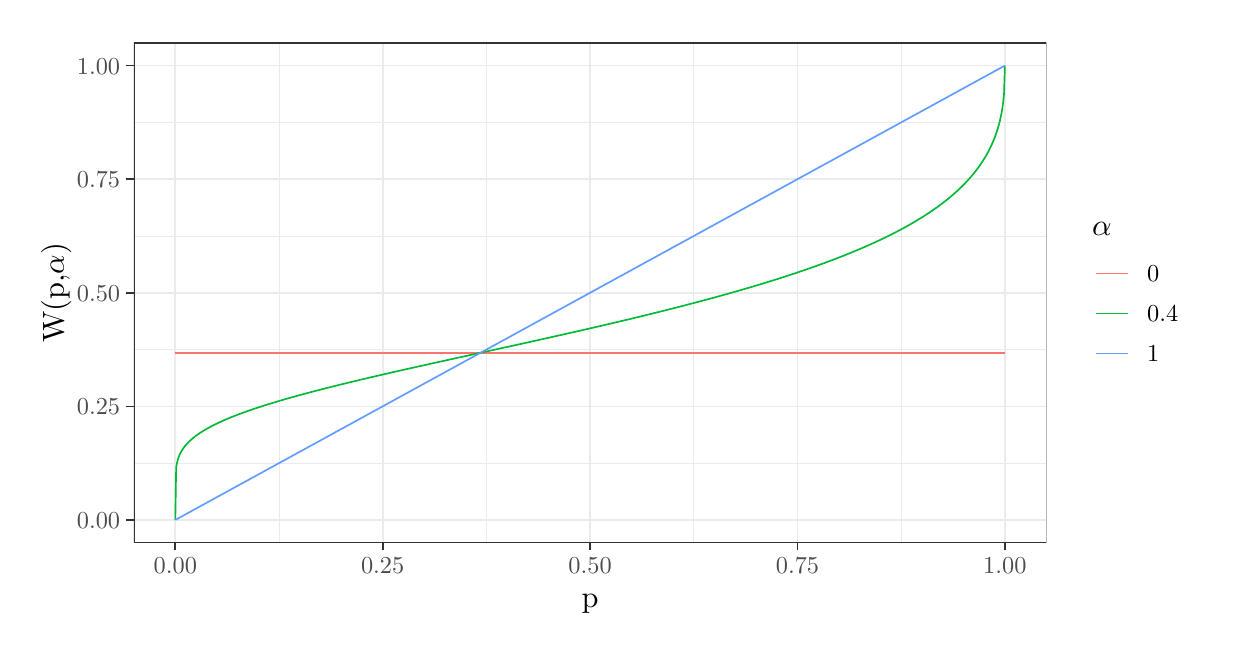
\begin{tikzpicture}[x=1pt,y=1pt]
\definecolor{fillColor}{RGB}{255,255,255}
\path[use as bounding box,fill=fillColor,fill opacity=0.00] (0,0) rectangle (426.79,216.81);
\begin{scope}
\path[clip] (  0.00,  0.00) rectangle (426.79,216.81);
\definecolor{drawColor}{RGB}{255,255,255}
\definecolor{fillColor}{RGB}{255,255,255}

\path[draw=drawColor,line width= 0.6pt,line join=round,line cap=round,fill=fillColor] (  0.00,  0.00) rectangle (426.79,216.81);
\end{scope}
\begin{scope}
\path[clip] ( 38.36, 30.72) rectangle (368.10,211.31);
\definecolor{fillColor}{RGB}{255,255,255}

\path[fill=fillColor] ( 38.36, 30.72) rectangle (368.10,211.31);
\definecolor{drawColor}{gray}{0.92}

\path[draw=drawColor,line width= 0.3pt,line join=round] ( 38.36, 59.45) --
	(368.10, 59.45);

\path[draw=drawColor,line width= 0.3pt,line join=round] ( 38.36,100.50) --
	(368.10,100.50);

\path[draw=drawColor,line width= 0.3pt,line join=round] ( 38.36,141.54) --
	(368.10,141.54);

\path[draw=drawColor,line width= 0.3pt,line join=round] ( 38.36,182.58) --
	(368.10,182.58);

\path[draw=drawColor,line width= 0.3pt,line join=round] ( 90.82, 30.72) --
	( 90.82,211.31);

\path[draw=drawColor,line width= 0.3pt,line join=round] (165.76, 30.72) --
	(165.76,211.31);

\path[draw=drawColor,line width= 0.3pt,line join=round] (240.70, 30.72) --
	(240.70,211.31);

\path[draw=drawColor,line width= 0.3pt,line join=round] (315.64, 30.72) --
	(315.64,211.31);

\path[draw=drawColor,line width= 0.6pt,line join=round] ( 38.36, 38.93) --
	(368.10, 38.93);

\path[draw=drawColor,line width= 0.6pt,line join=round] ( 38.36, 79.98) --
	(368.10, 79.98);

\path[draw=drawColor,line width= 0.6pt,line join=round] ( 38.36,121.02) --
	(368.10,121.02);

\path[draw=drawColor,line width= 0.6pt,line join=round] ( 38.36,162.06) --
	(368.10,162.06);

\path[draw=drawColor,line width= 0.6pt,line join=round] ( 38.36,203.10) --
	(368.10,203.10);

\path[draw=drawColor,line width= 0.6pt,line join=round] ( 53.35, 30.72) --
	( 53.35,211.31);

\path[draw=drawColor,line width= 0.6pt,line join=round] (128.29, 30.72) --
	(128.29,211.31);

\path[draw=drawColor,line width= 0.6pt,line join=round] (203.23, 30.72) --
	(203.23,211.31);

\path[draw=drawColor,line width= 0.6pt,line join=round] (278.17, 30.72) --
	(278.17,211.31);

\path[draw=drawColor,line width= 0.6pt,line join=round] (353.11, 30.72) --
	(353.11,211.31);
\definecolor{drawColor}{RGB}{248,118,109}

\path[draw=drawColor,line width= 0.6pt,line join=round] ( 53.35, 99.33) --
	( 53.65, 99.33) --
	( 53.95, 99.33) --
	( 54.25, 99.33) --
	( 54.55, 99.33) --
	( 54.85, 99.33) --
	( 55.15, 99.33) --
	( 55.45, 99.33) --
	( 55.75, 99.33) --
	( 56.05, 99.33) --
	( 56.35, 99.33) --
	( 56.65, 99.33) --
	( 56.95, 99.33) --
	( 57.25, 99.33) --
	( 57.55, 99.33) --
	( 57.84, 99.33) --
	( 58.14, 99.33) --
	( 58.44, 99.33) --
	( 58.74, 99.33) --
	( 59.04, 99.33) --
	( 59.34, 99.33) --
	( 59.64, 99.33) --
	( 59.94, 99.33) --
	( 60.24, 99.33) --
	( 60.54, 99.33) --
	( 60.84, 99.33) --
	( 61.14, 99.33) --
	( 61.44, 99.33) --
	( 61.74, 99.33) --
	( 62.04, 99.33) --
	( 62.34, 99.33) --
	( 62.64, 99.33) --
	( 62.94, 99.33) --
	( 63.24, 99.33) --
	( 63.54, 99.33) --
	( 63.84, 99.33) --
	( 64.14, 99.33) --
	( 64.44, 99.33) --
	( 64.74, 99.33) --
	( 65.04, 99.33) --
	( 65.34, 99.33) --
	( 65.64, 99.33) --
	( 65.94, 99.33) --
	( 66.24, 99.33) --
	( 66.54, 99.33) --
	( 66.84, 99.33) --
	( 67.14, 99.33) --
	( 67.44, 99.33) --
	( 67.74, 99.33) --
	( 68.04, 99.33) --
	( 68.34, 99.33) --
	( 68.64, 99.33) --
	( 68.94, 99.33) --
	( 69.24, 99.33) --
	( 69.54, 99.33) --
	( 69.84, 99.33) --
	( 70.14, 99.33) --
	( 70.43, 99.33) --
	( 70.73, 99.33) --
	( 71.03, 99.33) --
	( 71.33, 99.33) --
	( 71.63, 99.33) --
	( 71.93, 99.33) --
	( 72.23, 99.33) --
	( 72.53, 99.33) --
	( 72.83, 99.33) --
	( 73.13, 99.33) --
	( 73.43, 99.33) --
	( 73.73, 99.33) --
	( 74.03, 99.33) --
	( 74.33, 99.33) --
	( 74.63, 99.33) --
	( 74.93, 99.33) --
	( 75.23, 99.33) --
	( 75.53, 99.33) --
	( 75.83, 99.33) --
	( 76.13, 99.33) --
	( 76.43, 99.33) --
	( 76.73, 99.33) --
	( 77.03, 99.33) --
	( 77.33, 99.33) --
	( 77.63, 99.33) --
	( 77.93, 99.33) --
	( 78.23, 99.33) --
	( 78.53, 99.33) --
	( 78.83, 99.33) --
	( 79.13, 99.33) --
	( 79.43, 99.33) --
	( 79.73, 99.33) --
	( 80.03, 99.33) --
	( 80.33, 99.33) --
	( 80.63, 99.33) --
	( 80.93, 99.33) --
	( 81.23, 99.33) --
	( 81.53, 99.33) --
	( 81.83, 99.33) --
	( 82.13, 99.33) --
	( 82.43, 99.33) --
	( 82.72, 99.33) --
	( 83.02, 99.33) --
	( 83.32, 99.33) --
	( 83.62, 99.33) --
	( 83.92, 99.33) --
	( 84.22, 99.33) --
	( 84.52, 99.33) --
	( 84.82, 99.33) --
	( 85.12, 99.33) --
	( 85.42, 99.33) --
	( 85.72, 99.33) --
	( 86.02, 99.33) --
	( 86.32, 99.33) --
	( 86.62, 99.33) --
	( 86.92, 99.33) --
	( 87.22, 99.33) --
	( 87.52, 99.33) --
	( 87.82, 99.33) --
	( 88.12, 99.33) --
	( 88.42, 99.33) --
	( 88.72, 99.33) --
	( 89.02, 99.33) --
	( 89.32, 99.33) --
	( 89.62, 99.33) --
	( 89.92, 99.33) --
	( 90.22, 99.33) --
	( 90.52, 99.33) --
	( 90.82, 99.33) --
	( 91.12, 99.33) --
	( 91.42, 99.33) --
	( 91.72, 99.33) --
	( 92.02, 99.33) --
	( 92.32, 99.33) --
	( 92.62, 99.33) --
	( 92.92, 99.33) --
	( 93.22, 99.33) --
	( 93.52, 99.33) --
	( 93.82, 99.33) --
	( 94.12, 99.33) --
	( 94.42, 99.33) --
	( 94.72, 99.33) --
	( 95.02, 99.33) --
	( 95.31, 99.33) --
	( 95.61, 99.33) --
	( 95.91, 99.33) --
	( 96.21, 99.33) --
	( 96.51, 99.33) --
	( 96.81, 99.33) --
	( 97.11, 99.33) --
	( 97.41, 99.33) --
	( 97.71, 99.33) --
	( 98.01, 99.33) --
	( 98.31, 99.33) --
	( 98.61, 99.33) --
	( 98.91, 99.33) --
	( 99.21, 99.33) --
	( 99.51, 99.33) --
	( 99.81, 99.33) --
	(100.11, 99.33) --
	(100.41, 99.33) --
	(100.71, 99.33) --
	(101.01, 99.33) --
	(101.31, 99.33) --
	(101.61, 99.33) --
	(101.91, 99.33) --
	(102.21, 99.33) --
	(102.51, 99.33) --
	(102.81, 99.33) --
	(103.11, 99.33) --
	(103.41, 99.33) --
	(103.71, 99.33) --
	(104.01, 99.33) --
	(104.31, 99.33) --
	(104.61, 99.33) --
	(104.91, 99.33) --
	(105.21, 99.33) --
	(105.51, 99.33) --
	(105.81, 99.33) --
	(106.11, 99.33) --
	(106.41, 99.33) --
	(106.71, 99.33) --
	(107.01, 99.33) --
	(107.31, 99.33) --
	(107.60, 99.33) --
	(107.90, 99.33) --
	(108.20, 99.33) --
	(108.50, 99.33) --
	(108.80, 99.33) --
	(109.10, 99.33) --
	(109.40, 99.33) --
	(109.70, 99.33) --
	(110.00, 99.33) --
	(110.30, 99.33) --
	(110.60, 99.33) --
	(110.90, 99.33) --
	(111.20, 99.33) --
	(111.50, 99.33) --
	(111.80, 99.33) --
	(112.10, 99.33) --
	(112.40, 99.33) --
	(112.70, 99.33) --
	(113.00, 99.33) --
	(113.30, 99.33) --
	(113.60, 99.33) --
	(113.90, 99.33) --
	(114.20, 99.33) --
	(114.50, 99.33) --
	(114.80, 99.33) --
	(115.10, 99.33) --
	(115.40, 99.33) --
	(115.70, 99.33) --
	(116.00, 99.33) --
	(116.30, 99.33) --
	(116.60, 99.33) --
	(116.90, 99.33) --
	(117.20, 99.33) --
	(117.50, 99.33) --
	(117.80, 99.33) --
	(118.10, 99.33) --
	(118.40, 99.33) --
	(118.70, 99.33) --
	(119.00, 99.33) --
	(119.30, 99.33) --
	(119.60, 99.33) --
	(119.90, 99.33) --
	(120.19, 99.33) --
	(120.49, 99.33) --
	(120.79, 99.33) --
	(121.09, 99.33) --
	(121.39, 99.33) --
	(121.69, 99.33) --
	(121.99, 99.33) --
	(122.29, 99.33) --
	(122.59, 99.33) --
	(122.89, 99.33) --
	(123.19, 99.33) --
	(123.49, 99.33) --
	(123.79, 99.33) --
	(124.09, 99.33) --
	(124.39, 99.33) --
	(124.69, 99.33) --
	(124.99, 99.33) --
	(125.29, 99.33) --
	(125.59, 99.33) --
	(125.89, 99.33) --
	(126.19, 99.33) --
	(126.49, 99.33) --
	(126.79, 99.33) --
	(127.09, 99.33) --
	(127.39, 99.33) --
	(127.69, 99.33) --
	(127.99, 99.33) --
	(128.29, 99.33) --
	(128.59, 99.33) --
	(128.89, 99.33) --
	(129.19, 99.33) --
	(129.49, 99.33) --
	(129.79, 99.33) --
	(130.09, 99.33) --
	(130.39, 99.33) --
	(130.69, 99.33) --
	(130.99, 99.33) --
	(131.29, 99.33) --
	(131.59, 99.33) --
	(131.89, 99.33) --
	(132.19, 99.33) --
	(132.48, 99.33) --
	(132.78, 99.33) --
	(133.08, 99.33) --
	(133.38, 99.33) --
	(133.68, 99.33) --
	(133.98, 99.33) --
	(134.28, 99.33) --
	(134.58, 99.33) --
	(134.88, 99.33) --
	(135.18, 99.33) --
	(135.48, 99.33) --
	(135.78, 99.33) --
	(136.08, 99.33) --
	(136.38, 99.33) --
	(136.68, 99.33) --
	(136.98, 99.33) --
	(137.28, 99.33) --
	(137.58, 99.33) --
	(137.88, 99.33) --
	(138.18, 99.33) --
	(138.48, 99.33) --
	(138.78, 99.33) --
	(139.08, 99.33) --
	(139.38, 99.33) --
	(139.68, 99.33) --
	(139.98, 99.33) --
	(140.28, 99.33) --
	(140.58, 99.33) --
	(140.88, 99.33) --
	(141.18, 99.33) --
	(141.48, 99.33) --
	(141.78, 99.33) --
	(142.08, 99.33) --
	(142.38, 99.33) --
	(142.68, 99.33) --
	(142.98, 99.33) --
	(143.28, 99.33) --
	(143.58, 99.33) --
	(143.88, 99.33) --
	(144.18, 99.33) --
	(144.48, 99.33) --
	(144.78, 99.33) --
	(145.07, 99.33) --
	(145.37, 99.33) --
	(145.67, 99.33) --
	(145.97, 99.33) --
	(146.27, 99.33) --
	(146.57, 99.33) --
	(146.87, 99.33) --
	(147.17, 99.33) --
	(147.47, 99.33) --
	(147.77, 99.33) --
	(148.07, 99.33) --
	(148.37, 99.33) --
	(148.67, 99.33) --
	(148.97, 99.33) --
	(149.27, 99.33) --
	(149.57, 99.33) --
	(149.87, 99.33) --
	(150.17, 99.33) --
	(150.47, 99.33) --
	(150.77, 99.33) --
	(151.07, 99.33) --
	(151.37, 99.33) --
	(151.67, 99.33) --
	(151.97, 99.33) --
	(152.27, 99.33) --
	(152.57, 99.33) --
	(152.87, 99.33) --
	(153.17, 99.33) --
	(153.47, 99.33) --
	(153.77, 99.33) --
	(154.07, 99.33) --
	(154.37, 99.33) --
	(154.67, 99.33) --
	(154.97, 99.33) --
	(155.27, 99.33) --
	(155.57, 99.33) --
	(155.87, 99.33) --
	(156.17, 99.33) --
	(156.47, 99.33) --
	(156.77, 99.33) --
	(157.07, 99.33) --
	(157.36, 99.33) --
	(157.66, 99.33) --
	(157.96, 99.33) --
	(158.26, 99.33) --
	(158.56, 99.33) --
	(158.86, 99.33) --
	(159.16, 99.33) --
	(159.46, 99.33) --
	(159.76, 99.33) --
	(160.06, 99.33) --
	(160.36, 99.33) --
	(160.66, 99.33) --
	(160.96, 99.33) --
	(161.26, 99.33) --
	(161.56, 99.33) --
	(161.86, 99.33) --
	(162.16, 99.33) --
	(162.46, 99.33) --
	(162.76, 99.33) --
	(163.06, 99.33) --
	(163.36, 99.33) --
	(163.66, 99.33) --
	(163.96, 99.33) --
	(164.26, 99.33) --
	(164.56, 99.33) --
	(164.86, 99.33) --
	(165.16, 99.33) --
	(165.46, 99.33) --
	(165.76, 99.33) --
	(166.06, 99.33) --
	(166.36, 99.33) --
	(166.66, 99.33) --
	(166.96, 99.33) --
	(167.26, 99.33) --
	(167.56, 99.33) --
	(167.86, 99.33) --
	(168.16, 99.33) --
	(168.46, 99.33) --
	(168.76, 99.33) --
	(169.06, 99.33) --
	(169.36, 99.33) --
	(169.66, 99.33) --
	(169.95, 99.33) --
	(170.25, 99.33) --
	(170.55, 99.33) --
	(170.85, 99.33) --
	(171.15, 99.33) --
	(171.45, 99.33) --
	(171.75, 99.33) --
	(172.05, 99.33) --
	(172.35, 99.33) --
	(172.65, 99.33) --
	(172.95, 99.33) --
	(173.25, 99.33) --
	(173.55, 99.33) --
	(173.85, 99.33) --
	(174.15, 99.33) --
	(174.45, 99.33) --
	(174.75, 99.33) --
	(175.05, 99.33) --
	(175.35, 99.33) --
	(175.65, 99.33) --
	(175.95, 99.33) --
	(176.25, 99.33) --
	(176.55, 99.33) --
	(176.85, 99.33) --
	(177.15, 99.33) --
	(177.45, 99.33) --
	(177.75, 99.33) --
	(178.05, 99.33) --
	(178.35, 99.33) --
	(178.65, 99.33) --
	(178.95, 99.33) --
	(179.25, 99.33) --
	(179.55, 99.33) --
	(179.85, 99.33) --
	(180.15, 99.33) --
	(180.45, 99.33) --
	(180.75, 99.33) --
	(181.05, 99.33) --
	(181.35, 99.33) --
	(181.65, 99.33) --
	(181.95, 99.33) --
	(182.24, 99.33) --
	(182.54, 99.33) --
	(182.84, 99.33) --
	(183.14, 99.33) --
	(183.44, 99.33) --
	(183.74, 99.33) --
	(184.04, 99.33) --
	(184.34, 99.33) --
	(184.64, 99.33) --
	(184.94, 99.33) --
	(185.24, 99.33) --
	(185.54, 99.33) --
	(185.84, 99.33) --
	(186.14, 99.33) --
	(186.44, 99.33) --
	(186.74, 99.33) --
	(187.04, 99.33) --
	(187.34, 99.33) --
	(187.64, 99.33) --
	(187.94, 99.33) --
	(188.24, 99.33) --
	(188.54, 99.33) --
	(188.84, 99.33) --
	(189.14, 99.33) --
	(189.44, 99.33) --
	(189.74, 99.33) --
	(190.04, 99.33) --
	(190.34, 99.33) --
	(190.64, 99.33) --
	(190.94, 99.33) --
	(191.24, 99.33) --
	(191.54, 99.33) --
	(191.84, 99.33) --
	(192.14, 99.33) --
	(192.44, 99.33) --
	(192.74, 99.33) --
	(193.04, 99.33) --
	(193.34, 99.33) --
	(193.64, 99.33) --
	(193.94, 99.33) --
	(194.24, 99.33) --
	(194.54, 99.33) --
	(194.83, 99.33) --
	(195.13, 99.33) --
	(195.43, 99.33) --
	(195.73, 99.33) --
	(196.03, 99.33) --
	(196.33, 99.33) --
	(196.63, 99.33) --
	(196.93, 99.33) --
	(197.23, 99.33) --
	(197.53, 99.33) --
	(197.83, 99.33) --
	(198.13, 99.33) --
	(198.43, 99.33) --
	(198.73, 99.33) --
	(199.03, 99.33) --
	(199.33, 99.33) --
	(199.63, 99.33) --
	(199.93, 99.33) --
	(200.23, 99.33) --
	(200.53, 99.33) --
	(200.83, 99.33) --
	(201.13, 99.33) --
	(201.43, 99.33) --
	(201.73, 99.33) --
	(202.03, 99.33) --
	(202.33, 99.33) --
	(202.63, 99.33) --
	(202.93, 99.33) --
	(203.23, 99.33) --
	(203.53, 99.33) --
	(203.83, 99.33) --
	(204.13, 99.33) --
	(204.43, 99.33) --
	(204.73, 99.33) --
	(205.03, 99.33) --
	(205.33, 99.33) --
	(205.63, 99.33) --
	(205.93, 99.33) --
	(206.23, 99.33) --
	(206.53, 99.33) --
	(206.83, 99.33) --
	(207.12, 99.33) --
	(207.42, 99.33) --
	(207.72, 99.33) --
	(208.02, 99.33) --
	(208.32, 99.33) --
	(208.62, 99.33) --
	(208.92, 99.33) --
	(209.22, 99.33) --
	(209.52, 99.33) --
	(209.82, 99.33) --
	(210.12, 99.33) --
	(210.42, 99.33) --
	(210.72, 99.33) --
	(211.02, 99.33) --
	(211.32, 99.33) --
	(211.62, 99.33) --
	(211.92, 99.33) --
	(212.22, 99.33) --
	(212.52, 99.33) --
	(212.82, 99.33) --
	(213.12, 99.33) --
	(213.42, 99.33) --
	(213.72, 99.33) --
	(214.02, 99.33) --
	(214.32, 99.33) --
	(214.62, 99.33) --
	(214.92, 99.33) --
	(215.22, 99.33) --
	(215.52, 99.33) --
	(215.82, 99.33) --
	(216.12, 99.33) --
	(216.42, 99.33) --
	(216.72, 99.33) --
	(217.02, 99.33) --
	(217.32, 99.33) --
	(217.62, 99.33) --
	(217.92, 99.33) --
	(218.22, 99.33) --
	(218.52, 99.33) --
	(218.82, 99.33) --
	(219.12, 99.33) --
	(219.42, 99.33) --
	(219.71, 99.33) --
	(220.01, 99.33) --
	(220.31, 99.33) --
	(220.61, 99.33) --
	(220.91, 99.33) --
	(221.21, 99.33) --
	(221.51, 99.33) --
	(221.81, 99.33) --
	(222.11, 99.33) --
	(222.41, 99.33) --
	(222.71, 99.33) --
	(223.01, 99.33) --
	(223.31, 99.33) --
	(223.61, 99.33) --
	(223.91, 99.33) --
	(224.21, 99.33) --
	(224.51, 99.33) --
	(224.81, 99.33) --
	(225.11, 99.33) --
	(225.41, 99.33) --
	(225.71, 99.33) --
	(226.01, 99.33) --
	(226.31, 99.33) --
	(226.61, 99.33) --
	(226.91, 99.33) --
	(227.21, 99.33) --
	(227.51, 99.33) --
	(227.81, 99.33) --
	(228.11, 99.33) --
	(228.41, 99.33) --
	(228.71, 99.33) --
	(229.01, 99.33) --
	(229.31, 99.33) --
	(229.61, 99.33) --
	(229.91, 99.33) --
	(230.21, 99.33) --
	(230.51, 99.33) --
	(230.81, 99.33) --
	(231.11, 99.33) --
	(231.41, 99.33) --
	(231.71, 99.33) --
	(232.00, 99.33) --
	(232.30, 99.33) --
	(232.60, 99.33) --
	(232.90, 99.33) --
	(233.20, 99.33) --
	(233.50, 99.33) --
	(233.80, 99.33) --
	(234.10, 99.33) --
	(234.40, 99.33) --
	(234.70, 99.33) --
	(235.00, 99.33) --
	(235.30, 99.33) --
	(235.60, 99.33) --
	(235.90, 99.33) --
	(236.20, 99.33) --
	(236.50, 99.33) --
	(236.80, 99.33) --
	(237.10, 99.33) --
	(237.40, 99.33) --
	(237.70, 99.33) --
	(238.00, 99.33) --
	(238.30, 99.33) --
	(238.60, 99.33) --
	(238.90, 99.33) --
	(239.20, 99.33) --
	(239.50, 99.33) --
	(239.80, 99.33) --
	(240.10, 99.33) --
	(240.40, 99.33) --
	(240.70, 99.33) --
	(241.00, 99.33) --
	(241.30, 99.33) --
	(241.60, 99.33) --
	(241.90, 99.33) --
	(242.20, 99.33) --
	(242.50, 99.33) --
	(242.80, 99.33) --
	(243.10, 99.33) --
	(243.40, 99.33) --
	(243.70, 99.33) --
	(244.00, 99.33) --
	(244.30, 99.33) --
	(244.59, 99.33) --
	(244.89, 99.33) --
	(245.19, 99.33) --
	(245.49, 99.33) --
	(245.79, 99.33) --
	(246.09, 99.33) --
	(246.39, 99.33) --
	(246.69, 99.33) --
	(246.99, 99.33) --
	(247.29, 99.33) --
	(247.59, 99.33) --
	(247.89, 99.33) --
	(248.19, 99.33) --
	(248.49, 99.33) --
	(248.79, 99.33) --
	(249.09, 99.33) --
	(249.39, 99.33) --
	(249.69, 99.33) --
	(249.99, 99.33) --
	(250.29, 99.33) --
	(250.59, 99.33) --
	(250.89, 99.33) --
	(251.19, 99.33) --
	(251.49, 99.33) --
	(251.79, 99.33) --
	(252.09, 99.33) --
	(252.39, 99.33) --
	(252.69, 99.33) --
	(252.99, 99.33) --
	(253.29, 99.33) --
	(253.59, 99.33) --
	(253.89, 99.33) --
	(254.19, 99.33) --
	(254.49, 99.33) --
	(254.79, 99.33) --
	(255.09, 99.33) --
	(255.39, 99.33) --
	(255.69, 99.33) --
	(255.99, 99.33) --
	(256.29, 99.33) --
	(256.59, 99.33) --
	(256.88, 99.33) --
	(257.18, 99.33) --
	(257.48, 99.33) --
	(257.78, 99.33) --
	(258.08, 99.33) --
	(258.38, 99.33) --
	(258.68, 99.33) --
	(258.98, 99.33) --
	(259.28, 99.33) --
	(259.58, 99.33) --
	(259.88, 99.33) --
	(260.18, 99.33) --
	(260.48, 99.33) --
	(260.78, 99.33) --
	(261.08, 99.33) --
	(261.38, 99.33) --
	(261.68, 99.33) --
	(261.98, 99.33) --
	(262.28, 99.33) --
	(262.58, 99.33) --
	(262.88, 99.33) --
	(263.18, 99.33) --
	(263.48, 99.33) --
	(263.78, 99.33) --
	(264.08, 99.33) --
	(264.38, 99.33) --
	(264.68, 99.33) --
	(264.98, 99.33) --
	(265.28, 99.33) --
	(265.58, 99.33) --
	(265.88, 99.33) --
	(266.18, 99.33) --
	(266.48, 99.33) --
	(266.78, 99.33) --
	(267.08, 99.33) --
	(267.38, 99.33) --
	(267.68, 99.33) --
	(267.98, 99.33) --
	(268.28, 99.33) --
	(268.58, 99.33) --
	(268.88, 99.33) --
	(269.18, 99.33) --
	(269.47, 99.33) --
	(269.77, 99.33) --
	(270.07, 99.33) --
	(270.37, 99.33) --
	(270.67, 99.33) --
	(270.97, 99.33) --
	(271.27, 99.33) --
	(271.57, 99.33) --
	(271.87, 99.33) --
	(272.17, 99.33) --
	(272.47, 99.33) --
	(272.77, 99.33) --
	(273.07, 99.33) --
	(273.37, 99.33) --
	(273.67, 99.33) --
	(273.97, 99.33) --
	(274.27, 99.33) --
	(274.57, 99.33) --
	(274.87, 99.33) --
	(275.17, 99.33) --
	(275.47, 99.33) --
	(275.77, 99.33) --
	(276.07, 99.33) --
	(276.37, 99.33) --
	(276.67, 99.33) --
	(276.97, 99.33) --
	(277.27, 99.33) --
	(277.57, 99.33) --
	(277.87, 99.33) --
	(278.17, 99.33) --
	(278.47, 99.33) --
	(278.77, 99.33) --
	(279.07, 99.33) --
	(279.37, 99.33) --
	(279.67, 99.33) --
	(279.97, 99.33) --
	(280.27, 99.33) --
	(280.57, 99.33) --
	(280.87, 99.33) --
	(281.17, 99.33) --
	(281.47, 99.33) --
	(281.76, 99.33) --
	(282.06, 99.33) --
	(282.36, 99.33) --
	(282.66, 99.33) --
	(282.96, 99.33) --
	(283.26, 99.33) --
	(283.56, 99.33) --
	(283.86, 99.33) --
	(284.16, 99.33) --
	(284.46, 99.33) --
	(284.76, 99.33) --
	(285.06, 99.33) --
	(285.36, 99.33) --
	(285.66, 99.33) --
	(285.96, 99.33) --
	(286.26, 99.33) --
	(286.56, 99.33) --
	(286.86, 99.33) --
	(287.16, 99.33) --
	(287.46, 99.33) --
	(287.76, 99.33) --
	(288.06, 99.33) --
	(288.36, 99.33) --
	(288.66, 99.33) --
	(288.96, 99.33) --
	(289.26, 99.33) --
	(289.56, 99.33) --
	(289.86, 99.33) --
	(290.16, 99.33) --
	(290.46, 99.33) --
	(290.76, 99.33) --
	(291.06, 99.33) --
	(291.36, 99.33) --
	(291.66, 99.33) --
	(291.96, 99.33) --
	(292.26, 99.33) --
	(292.56, 99.33) --
	(292.86, 99.33) --
	(293.16, 99.33) --
	(293.46, 99.33) --
	(293.76, 99.33) --
	(294.05, 99.33) --
	(294.35, 99.33) --
	(294.65, 99.33) --
	(294.95, 99.33) --
	(295.25, 99.33) --
	(295.55, 99.33) --
	(295.85, 99.33) --
	(296.15, 99.33) --
	(296.45, 99.33) --
	(296.75, 99.33) --
	(297.05, 99.33) --
	(297.35, 99.33) --
	(297.65, 99.33) --
	(297.95, 99.33) --
	(298.25, 99.33) --
	(298.55, 99.33) --
	(298.85, 99.33) --
	(299.15, 99.33) --
	(299.45, 99.33) --
	(299.75, 99.33) --
	(300.05, 99.33) --
	(300.35, 99.33) --
	(300.65, 99.33) --
	(300.95, 99.33) --
	(301.25, 99.33) --
	(301.55, 99.33) --
	(301.85, 99.33) --
	(302.15, 99.33) --
	(302.45, 99.33) --
	(302.75, 99.33) --
	(303.05, 99.33) --
	(303.35, 99.33) --
	(303.65, 99.33) --
	(303.95, 99.33) --
	(304.25, 99.33) --
	(304.55, 99.33) --
	(304.85, 99.33) --
	(305.15, 99.33) --
	(305.45, 99.33) --
	(305.75, 99.33) --
	(306.05, 99.33) --
	(306.35, 99.33) --
	(306.64, 99.33) --
	(306.94, 99.33) --
	(307.24, 99.33) --
	(307.54, 99.33) --
	(307.84, 99.33) --
	(308.14, 99.33) --
	(308.44, 99.33) --
	(308.74, 99.33) --
	(309.04, 99.33) --
	(309.34, 99.33) --
	(309.64, 99.33) --
	(309.94, 99.33) --
	(310.24, 99.33) --
	(310.54, 99.33) --
	(310.84, 99.33) --
	(311.14, 99.33) --
	(311.44, 99.33) --
	(311.74, 99.33) --
	(312.04, 99.33) --
	(312.34, 99.33) --
	(312.64, 99.33) --
	(312.94, 99.33) --
	(313.24, 99.33) --
	(313.54, 99.33) --
	(313.84, 99.33) --
	(314.14, 99.33) --
	(314.44, 99.33) --
	(314.74, 99.33) --
	(315.04, 99.33) --
	(315.34, 99.33) --
	(315.64, 99.33) --
	(315.94, 99.33) --
	(316.24, 99.33) --
	(316.54, 99.33) --
	(316.84, 99.33) --
	(317.14, 99.33) --
	(317.44, 99.33) --
	(317.74, 99.33) --
	(318.04, 99.33) --
	(318.34, 99.33) --
	(318.64, 99.33) --
	(318.93, 99.33) --
	(319.23, 99.33) --
	(319.53, 99.33) --
	(319.83, 99.33) --
	(320.13, 99.33) --
	(320.43, 99.33) --
	(320.73, 99.33) --
	(321.03, 99.33) --
	(321.33, 99.33) --
	(321.63, 99.33) --
	(321.93, 99.33) --
	(322.23, 99.33) --
	(322.53, 99.33) --
	(322.83, 99.33) --
	(323.13, 99.33) --
	(323.43, 99.33) --
	(323.73, 99.33) --
	(324.03, 99.33) --
	(324.33, 99.33) --
	(324.63, 99.33) --
	(324.93, 99.33) --
	(325.23, 99.33) --
	(325.53, 99.33) --
	(325.83, 99.33) --
	(326.13, 99.33) --
	(326.43, 99.33) --
	(326.73, 99.33) --
	(327.03, 99.33) --
	(327.33, 99.33) --
	(327.63, 99.33) --
	(327.93, 99.33) --
	(328.23, 99.33) --
	(328.53, 99.33) --
	(328.83, 99.33) --
	(329.13, 99.33) --
	(329.43, 99.33) --
	(329.73, 99.33) --
	(330.03, 99.33) --
	(330.33, 99.33) --
	(330.63, 99.33) --
	(330.93, 99.33) --
	(331.23, 99.33) --
	(331.52, 99.33) --
	(331.82, 99.33) --
	(332.12, 99.33) --
	(332.42, 99.33) --
	(332.72, 99.33) --
	(333.02, 99.33) --
	(333.32, 99.33) --
	(333.62, 99.33) --
	(333.92, 99.33) --
	(334.22, 99.33) --
	(334.52, 99.33) --
	(334.82, 99.33) --
	(335.12, 99.33) --
	(335.42, 99.33) --
	(335.72, 99.33) --
	(336.02, 99.33) --
	(336.32, 99.33) --
	(336.62, 99.33) --
	(336.92, 99.33) --
	(337.22, 99.33) --
	(337.52, 99.33) --
	(337.82, 99.33) --
	(338.12, 99.33) --
	(338.42, 99.33) --
	(338.72, 99.33) --
	(339.02, 99.33) --
	(339.32, 99.33) --
	(339.62, 99.33) --
	(339.92, 99.33) --
	(340.22, 99.33) --
	(340.52, 99.33) --
	(340.82, 99.33) --
	(341.12, 99.33) --
	(341.42, 99.33) --
	(341.72, 99.33) --
	(342.02, 99.33) --
	(342.32, 99.33) --
	(342.62, 99.33) --
	(342.92, 99.33) --
	(343.22, 99.33) --
	(343.52, 99.33) --
	(343.81, 99.33) --
	(344.11, 99.33) --
	(344.41, 99.33) --
	(344.71, 99.33) --
	(345.01, 99.33) --
	(345.31, 99.33) --
	(345.61, 99.33) --
	(345.91, 99.33) --
	(346.21, 99.33) --
	(346.51, 99.33) --
	(346.81, 99.33) --
	(347.11, 99.33) --
	(347.41, 99.33) --
	(347.71, 99.33) --
	(348.01, 99.33) --
	(348.31, 99.33) --
	(348.61, 99.33) --
	(348.91, 99.33) --
	(349.21, 99.33) --
	(349.51, 99.33) --
	(349.81, 99.33) --
	(350.11, 99.33) --
	(350.41, 99.33) --
	(350.71, 99.33) --
	(351.01, 99.33) --
	(351.31, 99.33) --
	(351.61, 99.33) --
	(351.91, 99.33) --
	(352.21, 99.33) --
	(352.51, 99.33) --
	(352.81, 99.33) --
	(353.11, 99.33);
\definecolor{drawColor}{RGB}{0,186,56}

\path[draw=drawColor,line width= 0.6pt,line join=round] ( 53.35, 38.93) --
	( 53.65, 57.75) --
	( 53.95, 59.51) --
	( 54.25, 60.68) --
	( 54.55, 61.58) --
	( 54.85, 62.33) --
	( 55.15, 62.97) --
	( 55.45, 63.54) --
	( 55.75, 64.05) --
	( 56.05, 64.52) --
	( 56.35, 64.95) --
	( 56.65, 65.36) --
	( 56.95, 65.73) --
	( 57.25, 66.09) --
	( 57.55, 66.43) --
	( 57.84, 66.75) --
	( 58.14, 67.05) --
	( 58.44, 67.35) --
	( 58.74, 67.63) --
	( 59.04, 67.90) --
	( 59.34, 68.16) --
	( 59.64, 68.42) --
	( 59.94, 68.66) --
	( 60.24, 68.90) --
	( 60.54, 69.13) --
	( 60.84, 69.36) --
	( 61.14, 69.58) --
	( 61.44, 69.79) --
	( 61.74, 70.00) --
	( 62.04, 70.21) --
	( 62.34, 70.41) --
	( 62.64, 70.60) --
	( 62.94, 70.79) --
	( 63.24, 70.98) --
	( 63.54, 71.16) --
	( 63.84, 71.35) --
	( 64.14, 71.52) --
	( 64.44, 71.70) --
	( 64.74, 71.87) --
	( 65.04, 72.04) --
	( 65.34, 72.21) --
	( 65.64, 72.37) --
	( 65.94, 72.53) --
	( 66.24, 72.69) --
	( 66.54, 72.85) --
	( 66.84, 73.00) --
	( 67.14, 73.15) --
	( 67.44, 73.30) --
	( 67.74, 73.45) --
	( 68.04, 73.60) --
	( 68.34, 73.74) --
	( 68.64, 73.89) --
	( 68.94, 74.03) --
	( 69.24, 74.17) --
	( 69.54, 74.31) --
	( 69.84, 74.44) --
	( 70.14, 74.58) --
	( 70.43, 74.71) --
	( 70.73, 74.85) --
	( 71.03, 74.98) --
	( 71.33, 75.11) --
	( 71.63, 75.24) --
	( 71.93, 75.37) --
	( 72.23, 75.49) --
	( 72.53, 75.62) --
	( 72.83, 75.74) --
	( 73.13, 75.87) --
	( 73.43, 75.99) --
	( 73.73, 76.11) --
	( 74.03, 76.23) --
	( 74.33, 76.35) --
	( 74.63, 76.47) --
	( 74.93, 76.59) --
	( 75.23, 76.70) --
	( 75.53, 76.82) --
	( 75.83, 76.93) --
	( 76.13, 77.05) --
	( 76.43, 77.16) --
	( 76.73, 77.27) --
	( 77.03, 77.38) --
	( 77.33, 77.50) --
	( 77.63, 77.61) --
	( 77.93, 77.72) --
	( 78.23, 77.82) --
	( 78.53, 77.93) --
	( 78.83, 78.04) --
	( 79.13, 78.15) --
	( 79.43, 78.25) --
	( 79.73, 78.36) --
	( 80.03, 78.46) --
	( 80.33, 78.57) --
	( 80.63, 78.67) --
	( 80.93, 78.77) --
	( 81.23, 78.88) --
	( 81.53, 78.98) --
	( 81.83, 79.08) --
	( 82.13, 79.18) --
	( 82.43, 79.28) --
	( 82.72, 79.38) --
	( 83.02, 79.48) --
	( 83.32, 79.58) --
	( 83.62, 79.68) --
	( 83.92, 79.77) --
	( 84.22, 79.87) --
	( 84.52, 79.97) --
	( 84.82, 80.07) --
	( 85.12, 80.16) --
	( 85.42, 80.26) --
	( 85.72, 80.35) --
	( 86.02, 80.45) --
	( 86.32, 80.54) --
	( 86.62, 80.64) --
	( 86.92, 80.73) --
	( 87.22, 80.82) --
	( 87.52, 80.91) --
	( 87.82, 81.01) --
	( 88.12, 81.10) --
	( 88.42, 81.19) --
	( 88.72, 81.28) --
	( 89.02, 81.37) --
	( 89.32, 81.46) --
	( 89.62, 81.55) --
	( 89.92, 81.64) --
	( 90.22, 81.73) --
	( 90.52, 81.82) --
	( 90.82, 81.91) --
	( 91.12, 82.00) --
	( 91.42, 82.09) --
	( 91.72, 82.17) --
	( 92.02, 82.26) --
	( 92.32, 82.35) --
	( 92.62, 82.44) --
	( 92.92, 82.52) --
	( 93.22, 82.61) --
	( 93.52, 82.70) --
	( 93.82, 82.78) --
	( 94.12, 82.87) --
	( 94.42, 82.95) --
	( 94.72, 83.04) --
	( 95.02, 83.12) --
	( 95.31, 83.21) --
	( 95.61, 83.29) --
	( 95.91, 83.37) --
	( 96.21, 83.46) --
	( 96.51, 83.54) --
	( 96.81, 83.62) --
	( 97.11, 83.71) --
	( 97.41, 83.79) --
	( 97.71, 83.87) --
	( 98.01, 83.95) --
	( 98.31, 84.04) --
	( 98.61, 84.12) --
	( 98.91, 84.20) --
	( 99.21, 84.28) --
	( 99.51, 84.36) --
	( 99.81, 84.44) --
	(100.11, 84.52) --
	(100.41, 84.60) --
	(100.71, 84.69) --
	(101.01, 84.77) --
	(101.31, 84.85) --
	(101.61, 84.92) --
	(101.91, 85.00) --
	(102.21, 85.08) --
	(102.51, 85.16) --
	(102.81, 85.24) --
	(103.11, 85.32) --
	(103.41, 85.40) --
	(103.71, 85.48) --
	(104.01, 85.56) --
	(104.31, 85.63) --
	(104.61, 85.71) --
	(104.91, 85.79) --
	(105.21, 85.87) --
	(105.51, 85.94) --
	(105.81, 86.02) --
	(106.11, 86.10) --
	(106.41, 86.18) --
	(106.71, 86.25) --
	(107.01, 86.33) --
	(107.31, 86.41) --
	(107.60, 86.48) --
	(107.90, 86.56) --
	(108.20, 86.63) --
	(108.50, 86.71) --
	(108.80, 86.78) --
	(109.10, 86.86) --
	(109.40, 86.94) --
	(109.70, 87.01) --
	(110.00, 87.09) --
	(110.30, 87.16) --
	(110.60, 87.24) --
	(110.90, 87.31) --
	(111.20, 87.39) --
	(111.50, 87.46) --
	(111.80, 87.53) --
	(112.10, 87.61) --
	(112.40, 87.68) --
	(112.70, 87.76) --
	(113.00, 87.83) --
	(113.30, 87.90) --
	(113.60, 87.98) --
	(113.90, 88.05) --
	(114.20, 88.12) --
	(114.50, 88.20) --
	(114.80, 88.27) --
	(115.10, 88.34) --
	(115.40, 88.42) --
	(115.70, 88.49) --
	(116.00, 88.56) --
	(116.30, 88.63) --
	(116.60, 88.71) --
	(116.90, 88.78) --
	(117.20, 88.85) --
	(117.50, 88.92) --
	(117.80, 88.99) --
	(118.10, 89.07) --
	(118.40, 89.14) --
	(118.70, 89.21) --
	(119.00, 89.28) --
	(119.30, 89.35) --
	(119.60, 89.42) --
	(119.90, 89.50) --
	(120.19, 89.57) --
	(120.49, 89.64) --
	(120.79, 89.71) --
	(121.09, 89.78) --
	(121.39, 89.85) --
	(121.69, 89.92) --
	(121.99, 89.99) --
	(122.29, 90.06) --
	(122.59, 90.13) --
	(122.89, 90.20) --
	(123.19, 90.28) --
	(123.49, 90.35) --
	(123.79, 90.42) --
	(124.09, 90.49) --
	(124.39, 90.56) --
	(124.69, 90.63) --
	(124.99, 90.70) --
	(125.29, 90.77) --
	(125.59, 90.84) --
	(125.89, 90.90) --
	(126.19, 90.97) --
	(126.49, 91.04) --
	(126.79, 91.11) --
	(127.09, 91.18) --
	(127.39, 91.25) --
	(127.69, 91.32) --
	(127.99, 91.39) --
	(128.29, 91.46) --
	(128.59, 91.53) --
	(128.89, 91.60) --
	(129.19, 91.67) --
	(129.49, 91.74) --
	(129.79, 91.80) --
	(130.09, 91.87) --
	(130.39, 91.94) --
	(130.69, 92.01) --
	(130.99, 92.08) --
	(131.29, 92.15) --
	(131.59, 92.22) --
	(131.89, 92.28) --
	(132.19, 92.35) --
	(132.48, 92.42) --
	(132.78, 92.49) --
	(133.08, 92.56) --
	(133.38, 92.63) --
	(133.68, 92.69) --
	(133.98, 92.76) --
	(134.28, 92.83) --
	(134.58, 92.90) --
	(134.88, 92.97) --
	(135.18, 93.03) --
	(135.48, 93.10) --
	(135.78, 93.17) --
	(136.08, 93.24) --
	(136.38, 93.30) --
	(136.68, 93.37) --
	(136.98, 93.44) --
	(137.28, 93.51) --
	(137.58, 93.57) --
	(137.88, 93.64) --
	(138.18, 93.71) --
	(138.48, 93.78) --
	(138.78, 93.84) --
	(139.08, 93.91) --
	(139.38, 93.98) --
	(139.68, 94.04) --
	(139.98, 94.11) --
	(140.28, 94.18) --
	(140.58, 94.25) --
	(140.88, 94.31) --
	(141.18, 94.38) --
	(141.48, 94.45) --
	(141.78, 94.51) --
	(142.08, 94.58) --
	(142.38, 94.65) --
	(142.68, 94.71) --
	(142.98, 94.78) --
	(143.28, 94.85) --
	(143.58, 94.91) --
	(143.88, 94.98) --
	(144.18, 95.05) --
	(144.48, 95.11) --
	(144.78, 95.18) --
	(145.07, 95.25) --
	(145.37, 95.31) --
	(145.67, 95.38) --
	(145.97, 95.45) --
	(146.27, 95.51) --
	(146.57, 95.58) --
	(146.87, 95.65) --
	(147.17, 95.71) --
	(147.47, 95.78) --
	(147.77, 95.84) --
	(148.07, 95.91) --
	(148.37, 95.98) --
	(148.67, 96.04) --
	(148.97, 96.11) --
	(149.27, 96.18) --
	(149.57, 96.24) --
	(149.87, 96.31) --
	(150.17, 96.37) --
	(150.47, 96.44) --
	(150.77, 96.51) --
	(151.07, 96.57) --
	(151.37, 96.64) --
	(151.67, 96.70) --
	(151.97, 96.77) --
	(152.27, 96.84) --
	(152.57, 96.90) --
	(152.87, 96.97) --
	(153.17, 97.03) --
	(153.47, 97.10) --
	(153.77, 97.17) --
	(154.07, 97.23) --
	(154.37, 97.30) --
	(154.67, 97.36) --
	(154.97, 97.43) --
	(155.27, 97.50) --
	(155.57, 97.56) --
	(155.87, 97.63) --
	(156.17, 97.69) --
	(156.47, 97.76) --
	(156.77, 97.82) --
	(157.07, 97.89) --
	(157.36, 97.96) --
	(157.66, 98.02) --
	(157.96, 98.09) --
	(158.26, 98.15) --
	(158.56, 98.22) --
	(158.86, 98.28) --
	(159.16, 98.35) --
	(159.46, 98.42) --
	(159.76, 98.48) --
	(160.06, 98.55) --
	(160.36, 98.61) --
	(160.66, 98.68) --
	(160.96, 98.74) --
	(161.26, 98.81) --
	(161.56, 98.88) --
	(161.86, 98.94) --
	(162.16, 99.01) --
	(162.46, 99.07) --
	(162.76, 99.14) --
	(163.06, 99.20) --
	(163.36, 99.27) --
	(163.66, 99.34) --
	(163.96, 99.40) --
	(164.26, 99.47) --
	(164.56, 99.53) --
	(164.86, 99.60) --
	(165.16, 99.66) --
	(165.46, 99.73) --
	(165.76, 99.79) --
	(166.06, 99.86) --
	(166.36, 99.93) --
	(166.66, 99.99) --
	(166.96,100.06) --
	(167.26,100.12) --
	(167.56,100.19) --
	(167.86,100.25) --
	(168.16,100.32) --
	(168.46,100.39) --
	(168.76,100.45) --
	(169.06,100.52) --
	(169.36,100.58) --
	(169.66,100.65) --
	(169.95,100.71) --
	(170.25,100.78) --
	(170.55,100.85) --
	(170.85,100.91) --
	(171.15,100.98) --
	(171.45,101.04) --
	(171.75,101.11) --
	(172.05,101.18) --
	(172.35,101.24) --
	(172.65,101.31) --
	(172.95,101.37) --
	(173.25,101.44) --
	(173.55,101.50) --
	(173.85,101.57) --
	(174.15,101.64) --
	(174.45,101.70) --
	(174.75,101.77) --
	(175.05,101.83) --
	(175.35,101.90) --
	(175.65,101.97) --
	(175.95,102.03) --
	(176.25,102.10) --
	(176.55,102.16) --
	(176.85,102.23) --
	(177.15,102.30) --
	(177.45,102.36) --
	(177.75,102.43) --
	(178.05,102.49) --
	(178.35,102.56) --
	(178.65,102.63) --
	(178.95,102.69) --
	(179.25,102.76) --
	(179.55,102.83) --
	(179.85,102.89) --
	(180.15,102.96) --
	(180.45,103.02) --
	(180.75,103.09) --
	(181.05,103.16) --
	(181.35,103.22) --
	(181.65,103.29) --
	(181.95,103.36) --
	(182.24,103.42) --
	(182.54,103.49) --
	(182.84,103.56) --
	(183.14,103.62) --
	(183.44,103.69) --
	(183.74,103.75) --
	(184.04,103.82) --
	(184.34,103.89) --
	(184.64,103.95) --
	(184.94,104.02) --
	(185.24,104.09) --
	(185.54,104.15) --
	(185.84,104.22) --
	(186.14,104.29) --
	(186.44,104.35) --
	(186.74,104.42) --
	(187.04,104.49) --
	(187.34,104.56) --
	(187.64,104.62) --
	(187.94,104.69) --
	(188.24,104.76) --
	(188.54,104.82) --
	(188.84,104.89) --
	(189.14,104.96) --
	(189.44,105.02) --
	(189.74,105.09) --
	(190.04,105.16) --
	(190.34,105.23) --
	(190.64,105.29) --
	(190.94,105.36) --
	(191.24,105.43) --
	(191.54,105.49) --
	(191.84,105.56) --
	(192.14,105.63) --
	(192.44,105.70) --
	(192.74,105.76) --
	(193.04,105.83) --
	(193.34,105.90) --
	(193.64,105.97) --
	(193.94,106.03) --
	(194.24,106.10) --
	(194.54,106.17) --
	(194.83,106.24) --
	(195.13,106.31) --
	(195.43,106.37) --
	(195.73,106.44) --
	(196.03,106.51) --
	(196.33,106.58) --
	(196.63,106.64) --
	(196.93,106.71) --
	(197.23,106.78) --
	(197.53,106.85) --
	(197.83,106.92) --
	(198.13,106.98) --
	(198.43,107.05) --
	(198.73,107.12) --
	(199.03,107.19) --
	(199.33,107.26) --
	(199.63,107.33) --
	(199.93,107.39) --
	(200.23,107.46) --
	(200.53,107.53) --
	(200.83,107.60) --
	(201.13,107.67) --
	(201.43,107.74) --
	(201.73,107.81) --
	(202.03,107.88) --
	(202.33,107.94) --
	(202.63,108.01) --
	(202.93,108.08) --
	(203.23,108.15) --
	(203.53,108.22) --
	(203.83,108.29) --
	(204.13,108.36) --
	(204.43,108.43) --
	(204.73,108.50) --
	(205.03,108.57) --
	(205.33,108.64) --
	(205.63,108.70) --
	(205.93,108.77) --
	(206.23,108.84) --
	(206.53,108.91) --
	(206.83,108.98) --
	(207.12,109.05) --
	(207.42,109.12) --
	(207.72,109.19) --
	(208.02,109.26) --
	(208.32,109.33) --
	(208.62,109.40) --
	(208.92,109.47) --
	(209.22,109.54) --
	(209.52,109.61) --
	(209.82,109.68) --
	(210.12,109.75) --
	(210.42,109.82) --
	(210.72,109.89) --
	(211.02,109.96) --
	(211.32,110.03) --
	(211.62,110.10) --
	(211.92,110.17) --
	(212.22,110.25) --
	(212.52,110.32) --
	(212.82,110.39) --
	(213.12,110.46) --
	(213.42,110.53) --
	(213.72,110.60) --
	(214.02,110.67) --
	(214.32,110.74) --
	(214.62,110.81) --
	(214.92,110.88) --
	(215.22,110.96) --
	(215.52,111.03) --
	(215.82,111.10) --
	(216.12,111.17) --
	(216.42,111.24) --
	(216.72,111.31) --
	(217.02,111.38) --
	(217.32,111.46) --
	(217.62,111.53) --
	(217.92,111.60) --
	(218.22,111.67) --
	(218.52,111.74) --
	(218.82,111.82) --
	(219.12,111.89) --
	(219.42,111.96) --
	(219.71,112.03) --
	(220.01,112.11) --
	(220.31,112.18) --
	(220.61,112.25) --
	(220.91,112.32) --
	(221.21,112.40) --
	(221.51,112.47) --
	(221.81,112.54) --
	(222.11,112.61) --
	(222.41,112.69) --
	(222.71,112.76) --
	(223.01,112.83) --
	(223.31,112.91) --
	(223.61,112.98) --
	(223.91,113.05) --
	(224.21,113.13) --
	(224.51,113.20) --
	(224.81,113.27) --
	(225.11,113.35) --
	(225.41,113.42) --
	(225.71,113.50) --
	(226.01,113.57) --
	(226.31,113.64) --
	(226.61,113.72) --
	(226.91,113.79) --
	(227.21,113.87) --
	(227.51,113.94) --
	(227.81,114.02) --
	(228.11,114.09) --
	(228.41,114.17) --
	(228.71,114.24) --
	(229.01,114.32) --
	(229.31,114.39) --
	(229.61,114.47) --
	(229.91,114.54) --
	(230.21,114.62) --
	(230.51,114.69) --
	(230.81,114.77) --
	(231.11,114.84) --
	(231.41,114.92) --
	(231.71,114.99) --
	(232.00,115.07) --
	(232.30,115.15) --
	(232.60,115.22) --
	(232.90,115.30) --
	(233.20,115.37) --
	(233.50,115.45) --
	(233.80,115.53) --
	(234.10,115.60) --
	(234.40,115.68) --
	(234.70,115.76) --
	(235.00,115.83) --
	(235.30,115.91) --
	(235.60,115.99) --
	(235.90,116.06) --
	(236.20,116.14) --
	(236.50,116.22) --
	(236.80,116.30) --
	(237.10,116.37) --
	(237.40,116.45) --
	(237.70,116.53) --
	(238.00,116.61) --
	(238.30,116.68) --
	(238.60,116.76) --
	(238.90,116.84) --
	(239.20,116.92) --
	(239.50,117.00) --
	(239.80,117.08) --
	(240.10,117.15) --
	(240.40,117.23) --
	(240.70,117.31) --
	(241.00,117.39) --
	(241.30,117.47) --
	(241.60,117.55) --
	(241.90,117.63) --
	(242.20,117.71) --
	(242.50,117.79) --
	(242.80,117.87) --
	(243.10,117.95) --
	(243.40,118.03) --
	(243.70,118.11) --
	(244.00,118.19) --
	(244.30,118.27) --
	(244.59,118.35) --
	(244.89,118.43) --
	(245.19,118.51) --
	(245.49,118.59) --
	(245.79,118.67) --
	(246.09,118.75) --
	(246.39,118.83) --
	(246.69,118.91) --
	(246.99,119.00) --
	(247.29,119.08) --
	(247.59,119.16) --
	(247.89,119.24) --
	(248.19,119.32) --
	(248.49,119.40) --
	(248.79,119.49) --
	(249.09,119.57) --
	(249.39,119.65) --
	(249.69,119.73) --
	(249.99,119.82) --
	(250.29,119.90) --
	(250.59,119.98) --
	(250.89,120.07) --
	(251.19,120.15) --
	(251.49,120.23) --
	(251.79,120.32) --
	(252.09,120.40) --
	(252.39,120.48) --
	(252.69,120.57) --
	(252.99,120.65) --
	(253.29,120.74) --
	(253.59,120.82) --
	(253.89,120.91) --
	(254.19,120.99) --
	(254.49,121.08) --
	(254.79,121.16) --
	(255.09,121.25) --
	(255.39,121.33) --
	(255.69,121.42) --
	(255.99,121.50) --
	(256.29,121.59) --
	(256.59,121.67) --
	(256.88,121.76) --
	(257.18,121.85) --
	(257.48,121.93) --
	(257.78,122.02) --
	(258.08,122.11) --
	(258.38,122.19) --
	(258.68,122.28) --
	(258.98,122.37) --
	(259.28,122.46) --
	(259.58,122.54) --
	(259.88,122.63) --
	(260.18,122.72) --
	(260.48,122.81) --
	(260.78,122.89) --
	(261.08,122.98) --
	(261.38,123.07) --
	(261.68,123.16) --
	(261.98,123.25) --
	(262.28,123.34) --
	(262.58,123.43) --
	(262.88,123.52) --
	(263.18,123.61) --
	(263.48,123.70) --
	(263.78,123.79) --
	(264.08,123.88) --
	(264.38,123.97) --
	(264.68,124.06) --
	(264.98,124.15) --
	(265.28,124.24) --
	(265.58,124.33) --
	(265.88,124.42) --
	(266.18,124.52) --
	(266.48,124.61) --
	(266.78,124.70) --
	(267.08,124.79) --
	(267.38,124.88) --
	(267.68,124.98) --
	(267.98,125.07) --
	(268.28,125.16) --
	(268.58,125.26) --
	(268.88,125.35) --
	(269.18,125.44) --
	(269.47,125.54) --
	(269.77,125.63) --
	(270.07,125.72) --
	(270.37,125.82) --
	(270.67,125.91) --
	(270.97,126.01) --
	(271.27,126.10) --
	(271.57,126.20) --
	(271.87,126.29) --
	(272.17,126.39) --
	(272.47,126.49) --
	(272.77,126.58) --
	(273.07,126.68) --
	(273.37,126.78) --
	(273.67,126.87) --
	(273.97,126.97) --
	(274.27,127.07) --
	(274.57,127.16) --
	(274.87,127.26) --
	(275.17,127.36) --
	(275.47,127.46) --
	(275.77,127.56) --
	(276.07,127.66) --
	(276.37,127.76) --
	(276.67,127.85) --
	(276.97,127.95) --
	(277.27,128.05) --
	(277.57,128.15) --
	(277.87,128.25) --
	(278.17,128.36) --
	(278.47,128.46) --
	(278.77,128.56) --
	(279.07,128.66) --
	(279.37,128.76) --
	(279.67,128.86) --
	(279.97,128.96) --
	(280.27,129.07) --
	(280.57,129.17) --
	(280.87,129.27) --
	(281.17,129.38) --
	(281.47,129.48) --
	(281.76,129.58) --
	(282.06,129.69) --
	(282.36,129.79) --
	(282.66,129.90) --
	(282.96,130.00) --
	(283.26,130.11) --
	(283.56,130.21) --
	(283.86,130.32) --
	(284.16,130.42) --
	(284.46,130.53) --
	(284.76,130.64) --
	(285.06,130.74) --
	(285.36,130.85) --
	(285.66,130.96) --
	(285.96,131.07) --
	(286.26,131.18) --
	(286.56,131.28) --
	(286.86,131.39) --
	(287.16,131.50) --
	(287.46,131.61) --
	(287.76,131.72) --
	(288.06,131.83) --
	(288.36,131.94) --
	(288.66,132.05) --
	(288.96,132.17) --
	(289.26,132.28) --
	(289.56,132.39) --
	(289.86,132.50) --
	(290.16,132.61) --
	(290.46,132.73) --
	(290.76,132.84) --
	(291.06,132.95) --
	(291.36,133.07) --
	(291.66,133.18) --
	(291.96,133.30) --
	(292.26,133.41) --
	(292.56,133.53) --
	(292.86,133.65) --
	(293.16,133.76) --
	(293.46,133.88) --
	(293.76,134.00) --
	(294.05,134.11) --
	(294.35,134.23) --
	(294.65,134.35) --
	(294.95,134.47) --
	(295.25,134.59) --
	(295.55,134.71) --
	(295.85,134.83) --
	(296.15,134.95) --
	(296.45,135.07) --
	(296.75,135.19) --
	(297.05,135.31) --
	(297.35,135.43) --
	(297.65,135.56) --
	(297.95,135.68) --
	(298.25,135.80) --
	(298.55,135.93) --
	(298.85,136.05) --
	(299.15,136.18) --
	(299.45,136.30) --
	(299.75,136.43) --
	(300.05,136.55) --
	(300.35,136.68) --
	(300.65,136.81) --
	(300.95,136.94) --
	(301.25,137.06) --
	(301.55,137.19) --
	(301.85,137.32) --
	(302.15,137.45) --
	(302.45,137.58) --
	(302.75,137.71) --
	(303.05,137.85) --
	(303.35,137.98) --
	(303.65,138.11) --
	(303.95,138.24) --
	(304.25,138.38) --
	(304.55,138.51) --
	(304.85,138.65) --
	(305.15,138.78) --
	(305.45,138.92) --
	(305.75,139.05) --
	(306.05,139.19) --
	(306.35,139.33) --
	(306.64,139.47) --
	(306.94,139.61) --
	(307.24,139.74) --
	(307.54,139.88) --
	(307.84,140.03) --
	(308.14,140.17) --
	(308.44,140.31) --
	(308.74,140.45) --
	(309.04,140.59) --
	(309.34,140.74) --
	(309.64,140.88) --
	(309.94,141.03) --
	(310.24,141.18) --
	(310.54,141.32) --
	(310.84,141.47) --
	(311.14,141.62) --
	(311.44,141.77) --
	(311.74,141.92) --
	(312.04,142.07) --
	(312.34,142.22) --
	(312.64,142.37) --
	(312.94,142.52) --
	(313.24,142.68) --
	(313.54,142.83) --
	(313.84,142.99) --
	(314.14,143.14) --
	(314.44,143.30) --
	(314.74,143.46) --
	(315.04,143.61) --
	(315.34,143.77) --
	(315.64,143.93) --
	(315.94,144.10) --
	(316.24,144.26) --
	(316.54,144.42) --
	(316.84,144.58) --
	(317.14,144.75) --
	(317.44,144.91) --
	(317.74,145.08) --
	(318.04,145.25) --
	(318.34,145.42) --
	(318.64,145.59) --
	(318.93,145.76) --
	(319.23,145.93) --
	(319.53,146.10) --
	(319.83,146.28) --
	(320.13,146.45) --
	(320.43,146.63) --
	(320.73,146.80) --
	(321.03,146.98) --
	(321.33,147.16) --
	(321.63,147.34) --
	(321.93,147.52) --
	(322.23,147.71) --
	(322.53,147.89) --
	(322.83,148.08) --
	(323.13,148.26) --
	(323.43,148.45) --
	(323.73,148.64) --
	(324.03,148.83) --
	(324.33,149.03) --
	(324.63,149.22) --
	(324.93,149.41) --
	(325.23,149.61) --
	(325.53,149.81) --
	(325.83,150.01) --
	(326.13,150.21) --
	(326.43,150.41) --
	(326.73,150.61) --
	(327.03,150.82) --
	(327.33,151.03) --
	(327.63,151.24) --
	(327.93,151.45) --
	(328.23,151.66) --
	(328.53,151.87) --
	(328.83,152.09) --
	(329.13,152.31) --
	(329.43,152.53) --
	(329.73,152.75) --
	(330.03,152.97) --
	(330.33,153.20) --
	(330.63,153.43) --
	(330.93,153.66) --
	(331.23,153.89) --
	(331.52,154.12) --
	(331.82,154.36) --
	(332.12,154.60) --
	(332.42,154.84) --
	(332.72,155.08) --
	(333.02,155.33) --
	(333.32,155.58) --
	(333.62,155.83) --
	(333.92,156.08) --
	(334.22,156.34) --
	(334.52,156.60) --
	(334.82,156.86) --
	(335.12,157.13) --
	(335.42,157.40) --
	(335.72,157.67) --
	(336.02,157.94) --
	(336.32,158.22) --
	(336.62,158.50) --
	(336.92,158.79) --
	(337.22,159.08) --
	(337.52,159.37) --
	(337.82,159.67) --
	(338.12,159.97) --
	(338.42,160.27) --
	(338.72,160.58) --
	(339.02,160.90) --
	(339.32,161.22) --
	(339.62,161.54) --
	(339.92,161.87) --
	(340.22,162.20) --
	(340.52,162.54) --
	(340.82,162.88) --
	(341.12,163.23) --
	(341.42,163.59) --
	(341.72,163.95) --
	(342.02,164.32) --
	(342.32,164.70) --
	(342.62,165.08) --
	(342.92,165.47) --
	(343.22,165.87) --
	(343.52,166.27) --
	(343.81,166.69) --
	(344.11,167.11) --
	(344.41,167.55) --
	(344.71,167.99) --
	(345.01,168.45) --
	(345.31,168.92) --
	(345.61,169.40) --
	(345.91,169.89) --
	(346.21,170.39) --
	(346.51,170.92) --
	(346.81,171.45) --
	(347.11,172.01) --
	(347.41,172.58) --
	(347.71,173.18) --
	(348.01,173.80) --
	(348.31,174.44) --
	(348.61,175.11) --
	(348.91,175.81) --
	(349.21,176.54) --
	(349.51,177.31) --
	(349.81,178.13) --
	(350.11,179.00) --
	(350.41,179.92) --
	(350.71,180.92) --
	(351.01,182.00) --
	(351.31,183.18) --
	(351.61,184.50) --
	(351.91,186.01) --
	(352.21,187.78) --
	(352.51,189.98) --
	(352.81,193.06) --
	(353.11,203.10);
\definecolor{drawColor}{RGB}{97,156,255}

\path[draw=drawColor,line width= 0.6pt,line join=round] ( 53.35, 38.93) --
	( 53.65, 39.10) --
	( 53.95, 39.26) --
	( 54.25, 39.43) --
	( 54.55, 39.59) --
	( 54.85, 39.75) --
	( 55.15, 39.92) --
	( 55.45, 40.08) --
	( 55.75, 40.25) --
	( 56.05, 40.41) --
	( 56.35, 40.57) --
	( 56.65, 40.74) --
	( 56.95, 40.90) --
	( 57.25, 41.07) --
	( 57.55, 41.23) --
	( 57.84, 41.40) --
	( 58.14, 41.56) --
	( 58.44, 41.72) --
	( 58.74, 41.89) --
	( 59.04, 42.05) --
	( 59.34, 42.22) --
	( 59.64, 42.38) --
	( 59.94, 42.54) --
	( 60.24, 42.71) --
	( 60.54, 42.87) --
	( 60.84, 43.04) --
	( 61.14, 43.20) --
	( 61.44, 43.37) --
	( 61.74, 43.53) --
	( 62.04, 43.69) --
	( 62.34, 43.86) --
	( 62.64, 44.02) --
	( 62.94, 44.19) --
	( 63.24, 44.35) --
	( 63.54, 44.51) --
	( 63.84, 44.68) --
	( 64.14, 44.84) --
	( 64.44, 45.01) --
	( 64.74, 45.17) --
	( 65.04, 45.34) --
	( 65.34, 45.50) --
	( 65.64, 45.66) --
	( 65.94, 45.83) --
	( 66.24, 45.99) --
	( 66.54, 46.16) --
	( 66.84, 46.32) --
	( 67.14, 46.48) --
	( 67.44, 46.65) --
	( 67.74, 46.81) --
	( 68.04, 46.98) --
	( 68.34, 47.14) --
	( 68.64, 47.31) --
	( 68.94, 47.47) --
	( 69.24, 47.63) --
	( 69.54, 47.80) --
	( 69.84, 47.96) --
	( 70.14, 48.13) --
	( 70.43, 48.29) --
	( 70.73, 48.45) --
	( 71.03, 48.62) --
	( 71.33, 48.78) --
	( 71.63, 48.95) --
	( 71.93, 49.11) --
	( 72.23, 49.28) --
	( 72.53, 49.44) --
	( 72.83, 49.60) --
	( 73.13, 49.77) --
	( 73.43, 49.93) --
	( 73.73, 50.10) --
	( 74.03, 50.26) --
	( 74.33, 50.42) --
	( 74.63, 50.59) --
	( 74.93, 50.75) --
	( 75.23, 50.92) --
	( 75.53, 51.08) --
	( 75.83, 51.25) --
	( 76.13, 51.41) --
	( 76.43, 51.57) --
	( 76.73, 51.74) --
	( 77.03, 51.90) --
	( 77.33, 52.07) --
	( 77.63, 52.23) --
	( 77.93, 52.39) --
	( 78.23, 52.56) --
	( 78.53, 52.72) --
	( 78.83, 52.89) --
	( 79.13, 53.05) --
	( 79.43, 53.22) --
	( 79.73, 53.38) --
	( 80.03, 53.54) --
	( 80.33, 53.71) --
	( 80.63, 53.87) --
	( 80.93, 54.04) --
	( 81.23, 54.20) --
	( 81.53, 54.36) --
	( 81.83, 54.53) --
	( 82.13, 54.69) --
	( 82.43, 54.86) --
	( 82.72, 55.02) --
	( 83.02, 55.19) --
	( 83.32, 55.35) --
	( 83.62, 55.51) --
	( 83.92, 55.68) --
	( 84.22, 55.84) --
	( 84.52, 56.01) --
	( 84.82, 56.17) --
	( 85.12, 56.33) --
	( 85.42, 56.50) --
	( 85.72, 56.66) --
	( 86.02, 56.83) --
	( 86.32, 56.99) --
	( 86.62, 57.16) --
	( 86.92, 57.32) --
	( 87.22, 57.48) --
	( 87.52, 57.65) --
	( 87.82, 57.81) --
	( 88.12, 57.98) --
	( 88.42, 58.14) --
	( 88.72, 58.30) --
	( 89.02, 58.47) --
	( 89.32, 58.63) --
	( 89.62, 58.80) --
	( 89.92, 58.96) --
	( 90.22, 59.13) --
	( 90.52, 59.29) --
	( 90.82, 59.45) --
	( 91.12, 59.62) --
	( 91.42, 59.78) --
	( 91.72, 59.95) --
	( 92.02, 60.11) --
	( 92.32, 60.28) --
	( 92.62, 60.44) --
	( 92.92, 60.60) --
	( 93.22, 60.77) --
	( 93.52, 60.93) --
	( 93.82, 61.10) --
	( 94.12, 61.26) --
	( 94.42, 61.42) --
	( 94.72, 61.59) --
	( 95.02, 61.75) --
	( 95.31, 61.92) --
	( 95.61, 62.08) --
	( 95.91, 62.25) --
	( 96.21, 62.41) --
	( 96.51, 62.57) --
	( 96.81, 62.74) --
	( 97.11, 62.90) --
	( 97.41, 63.07) --
	( 97.71, 63.23) --
	( 98.01, 63.39) --
	( 98.31, 63.56) --
	( 98.61, 63.72) --
	( 98.91, 63.89) --
	( 99.21, 64.05) --
	( 99.51, 64.22) --
	( 99.81, 64.38) --
	(100.11, 64.54) --
	(100.41, 64.71) --
	(100.71, 64.87) --
	(101.01, 65.04) --
	(101.31, 65.20) --
	(101.61, 65.36) --
	(101.91, 65.53) --
	(102.21, 65.69) --
	(102.51, 65.86) --
	(102.81, 66.02) --
	(103.11, 66.19) --
	(103.41, 66.35) --
	(103.71, 66.51) --
	(104.01, 66.68) --
	(104.31, 66.84) --
	(104.61, 67.01) --
	(104.91, 67.17) --
	(105.21, 67.33) --
	(105.51, 67.50) --
	(105.81, 67.66) --
	(106.11, 67.83) --
	(106.41, 67.99) --
	(106.71, 68.16) --
	(107.01, 68.32) --
	(107.31, 68.48) --
	(107.60, 68.65) --
	(107.90, 68.81) --
	(108.20, 68.98) --
	(108.50, 69.14) --
	(108.80, 69.30) --
	(109.10, 69.47) --
	(109.40, 69.63) --
	(109.70, 69.80) --
	(110.00, 69.96) --
	(110.30, 70.13) --
	(110.60, 70.29) --
	(110.90, 70.45) --
	(111.20, 70.62) --
	(111.50, 70.78) --
	(111.80, 70.95) --
	(112.10, 71.11) --
	(112.40, 71.27) --
	(112.70, 71.44) --
	(113.00, 71.60) --
	(113.30, 71.77) --
	(113.60, 71.93) --
	(113.90, 72.10) --
	(114.20, 72.26) --
	(114.50, 72.42) --
	(114.80, 72.59) --
	(115.10, 72.75) --
	(115.40, 72.92) --
	(115.70, 73.08) --
	(116.00, 73.24) --
	(116.30, 73.41) --
	(116.60, 73.57) --
	(116.90, 73.74) --
	(117.20, 73.90) --
	(117.50, 74.07) --
	(117.80, 74.23) --
	(118.10, 74.39) --
	(118.40, 74.56) --
	(118.70, 74.72) --
	(119.00, 74.89) --
	(119.30, 75.05) --
	(119.60, 75.21) --
	(119.90, 75.38) --
	(120.19, 75.54) --
	(120.49, 75.71) --
	(120.79, 75.87) --
	(121.09, 76.04) --
	(121.39, 76.20) --
	(121.69, 76.36) --
	(121.99, 76.53) --
	(122.29, 76.69) --
	(122.59, 76.86) --
	(122.89, 77.02) --
	(123.19, 77.18) --
	(123.49, 77.35) --
	(123.79, 77.51) --
	(124.09, 77.68) --
	(124.39, 77.84) --
	(124.69, 78.01) --
	(124.99, 78.17) --
	(125.29, 78.33) --
	(125.59, 78.50) --
	(125.89, 78.66) --
	(126.19, 78.83) --
	(126.49, 78.99) --
	(126.79, 79.15) --
	(127.09, 79.32) --
	(127.39, 79.48) --
	(127.69, 79.65) --
	(127.99, 79.81) --
	(128.29, 79.98) --
	(128.59, 80.14) --
	(128.89, 80.30) --
	(129.19, 80.47) --
	(129.49, 80.63) --
	(129.79, 80.80) --
	(130.09, 80.96) --
	(130.39, 81.12) --
	(130.69, 81.29) --
	(130.99, 81.45) --
	(131.29, 81.62) --
	(131.59, 81.78) --
	(131.89, 81.95) --
	(132.19, 82.11) --
	(132.48, 82.27) --
	(132.78, 82.44) --
	(133.08, 82.60) --
	(133.38, 82.77) --
	(133.68, 82.93) --
	(133.98, 83.09) --
	(134.28, 83.26) --
	(134.58, 83.42) --
	(134.88, 83.59) --
	(135.18, 83.75) --
	(135.48, 83.92) --
	(135.78, 84.08) --
	(136.08, 84.24) --
	(136.38, 84.41) --
	(136.68, 84.57) --
	(136.98, 84.74) --
	(137.28, 84.90) --
	(137.58, 85.06) --
	(137.88, 85.23) --
	(138.18, 85.39) --
	(138.48, 85.56) --
	(138.78, 85.72) --
	(139.08, 85.89) --
	(139.38, 86.05) --
	(139.68, 86.21) --
	(139.98, 86.38) --
	(140.28, 86.54) --
	(140.58, 86.71) --
	(140.88, 86.87) --
	(141.18, 87.03) --
	(141.48, 87.20) --
	(141.78, 87.36) --
	(142.08, 87.53) --
	(142.38, 87.69) --
	(142.68, 87.86) --
	(142.98, 88.02) --
	(143.28, 88.18) --
	(143.58, 88.35) --
	(143.88, 88.51) --
	(144.18, 88.68) --
	(144.48, 88.84) --
	(144.78, 89.00) --
	(145.07, 89.17) --
	(145.37, 89.33) --
	(145.67, 89.50) --
	(145.97, 89.66) --
	(146.27, 89.83) --
	(146.57, 89.99) --
	(146.87, 90.15) --
	(147.17, 90.32) --
	(147.47, 90.48) --
	(147.77, 90.65) --
	(148.07, 90.81) --
	(148.37, 90.97) --
	(148.67, 91.14) --
	(148.97, 91.30) --
	(149.27, 91.47) --
	(149.57, 91.63) --
	(149.87, 91.80) --
	(150.17, 91.96) --
	(150.47, 92.12) --
	(150.77, 92.29) --
	(151.07, 92.45) --
	(151.37, 92.62) --
	(151.67, 92.78) --
	(151.97, 92.94) --
	(152.27, 93.11) --
	(152.57, 93.27) --
	(152.87, 93.44) --
	(153.17, 93.60) --
	(153.47, 93.77) --
	(153.77, 93.93) --
	(154.07, 94.09) --
	(154.37, 94.26) --
	(154.67, 94.42) --
	(154.97, 94.59) --
	(155.27, 94.75) --
	(155.57, 94.91) --
	(155.87, 95.08) --
	(156.17, 95.24) --
	(156.47, 95.41) --
	(156.77, 95.57) --
	(157.07, 95.74) --
	(157.36, 95.90) --
	(157.66, 96.06) --
	(157.96, 96.23) --
	(158.26, 96.39) --
	(158.56, 96.56) --
	(158.86, 96.72) --
	(159.16, 96.88) --
	(159.46, 97.05) --
	(159.76, 97.21) --
	(160.06, 97.38) --
	(160.36, 97.54) --
	(160.66, 97.71) --
	(160.96, 97.87) --
	(161.26, 98.03) --
	(161.56, 98.20) --
	(161.86, 98.36) --
	(162.16, 98.53) --
	(162.46, 98.69) --
	(162.76, 98.85) --
	(163.06, 99.02) --
	(163.36, 99.18) --
	(163.66, 99.35) --
	(163.96, 99.51) --
	(164.26, 99.68) --
	(164.56, 99.84) --
	(164.86,100.00) --
	(165.16,100.17) --
	(165.46,100.33) --
	(165.76,100.50) --
	(166.06,100.66) --
	(166.36,100.82) --
	(166.66,100.99) --
	(166.96,101.15) --
	(167.26,101.32) --
	(167.56,101.48) --
	(167.86,101.65) --
	(168.16,101.81) --
	(168.46,101.97) --
	(168.76,102.14) --
	(169.06,102.30) --
	(169.36,102.47) --
	(169.66,102.63) --
	(169.95,102.79) --
	(170.25,102.96) --
	(170.55,103.12) --
	(170.85,103.29) --
	(171.15,103.45) --
	(171.45,103.62) --
	(171.75,103.78) --
	(172.05,103.94) --
	(172.35,104.11) --
	(172.65,104.27) --
	(172.95,104.44) --
	(173.25,104.60) --
	(173.55,104.76) --
	(173.85,104.93) --
	(174.15,105.09) --
	(174.45,105.26) --
	(174.75,105.42) --
	(175.05,105.59) --
	(175.35,105.75) --
	(175.65,105.91) --
	(175.95,106.08) --
	(176.25,106.24) --
	(176.55,106.41) --
	(176.85,106.57) --
	(177.15,106.73) --
	(177.45,106.90) --
	(177.75,107.06) --
	(178.05,107.23) --
	(178.35,107.39) --
	(178.65,107.56) --
	(178.95,107.72) --
	(179.25,107.88) --
	(179.55,108.05) --
	(179.85,108.21) --
	(180.15,108.38) --
	(180.45,108.54) --
	(180.75,108.70) --
	(181.05,108.87) --
	(181.35,109.03) --
	(181.65,109.20) --
	(181.95,109.36) --
	(182.24,109.53) --
	(182.54,109.69) --
	(182.84,109.85) --
	(183.14,110.02) --
	(183.44,110.18) --
	(183.74,110.35) --
	(184.04,110.51) --
	(184.34,110.67) --
	(184.64,110.84) --
	(184.94,111.00) --
	(185.24,111.17) --
	(185.54,111.33) --
	(185.84,111.50) --
	(186.14,111.66) --
	(186.44,111.82) --
	(186.74,111.99) --
	(187.04,112.15) --
	(187.34,112.32) --
	(187.64,112.48) --
	(187.94,112.64) --
	(188.24,112.81) --
	(188.54,112.97) --
	(188.84,113.14) --
	(189.14,113.30) --
	(189.44,113.47) --
	(189.74,113.63) --
	(190.04,113.79) --
	(190.34,113.96) --
	(190.64,114.12) --
	(190.94,114.29) --
	(191.24,114.45) --
	(191.54,114.61) --
	(191.84,114.78) --
	(192.14,114.94) --
	(192.44,115.11) --
	(192.74,115.27) --
	(193.04,115.44) --
	(193.34,115.60) --
	(193.64,115.76) --
	(193.94,115.93) --
	(194.24,116.09) --
	(194.54,116.26) --
	(194.83,116.42) --
	(195.13,116.58) --
	(195.43,116.75) --
	(195.73,116.91) --
	(196.03,117.08) --
	(196.33,117.24) --
	(196.63,117.41) --
	(196.93,117.57) --
	(197.23,117.73) --
	(197.53,117.90) --
	(197.83,118.06) --
	(198.13,118.23) --
	(198.43,118.39) --
	(198.73,118.55) --
	(199.03,118.72) --
	(199.33,118.88) --
	(199.63,119.05) --
	(199.93,119.21) --
	(200.23,119.38) --
	(200.53,119.54) --
	(200.83,119.70) --
	(201.13,119.87) --
	(201.43,120.03) --
	(201.73,120.20) --
	(202.03,120.36) --
	(202.33,120.52) --
	(202.63,120.69) --
	(202.93,120.85) --
	(203.23,121.02) --
	(203.53,121.18) --
	(203.83,121.35) --
	(204.13,121.51) --
	(204.43,121.67) --
	(204.73,121.84) --
	(205.03,122.00) --
	(205.33,122.17) --
	(205.63,122.33) --
	(205.93,122.49) --
	(206.23,122.66) --
	(206.53,122.82) --
	(206.83,122.99) --
	(207.12,123.15) --
	(207.42,123.32) --
	(207.72,123.48) --
	(208.02,123.64) --
	(208.32,123.81) --
	(208.62,123.97) --
	(208.92,124.14) --
	(209.22,124.30) --
	(209.52,124.46) --
	(209.82,124.63) --
	(210.12,124.79) --
	(210.42,124.96) --
	(210.72,125.12) --
	(211.02,125.29) --
	(211.32,125.45) --
	(211.62,125.61) --
	(211.92,125.78) --
	(212.22,125.94) --
	(212.52,126.11) --
	(212.82,126.27) --
	(213.12,126.43) --
	(213.42,126.60) --
	(213.72,126.76) --
	(214.02,126.93) --
	(214.32,127.09) --
	(214.62,127.26) --
	(214.92,127.42) --
	(215.22,127.58) --
	(215.52,127.75) --
	(215.82,127.91) --
	(216.12,128.08) --
	(216.42,128.24) --
	(216.72,128.40) --
	(217.02,128.57) --
	(217.32,128.73) --
	(217.62,128.90) --
	(217.92,129.06) --
	(218.22,129.23) --
	(218.52,129.39) --
	(218.82,129.55) --
	(219.12,129.72) --
	(219.42,129.88) --
	(219.71,130.05) --
	(220.01,130.21) --
	(220.31,130.37) --
	(220.61,130.54) --
	(220.91,130.70) --
	(221.21,130.87) --
	(221.51,131.03) --
	(221.81,131.20) --
	(222.11,131.36) --
	(222.41,131.52) --
	(222.71,131.69) --
	(223.01,131.85) --
	(223.31,132.02) --
	(223.61,132.18) --
	(223.91,132.34) --
	(224.21,132.51) --
	(224.51,132.67) --
	(224.81,132.84) --
	(225.11,133.00) --
	(225.41,133.17) --
	(225.71,133.33) --
	(226.01,133.49) --
	(226.31,133.66) --
	(226.61,133.82) --
	(226.91,133.99) --
	(227.21,134.15) --
	(227.51,134.31) --
	(227.81,134.48) --
	(228.11,134.64) --
	(228.41,134.81) --
	(228.71,134.97) --
	(229.01,135.14) --
	(229.31,135.30) --
	(229.61,135.46) --
	(229.91,135.63) --
	(230.21,135.79) --
	(230.51,135.96) --
	(230.81,136.12) --
	(231.11,136.29) --
	(231.41,136.45) --
	(231.71,136.61) --
	(232.00,136.78) --
	(232.30,136.94) --
	(232.60,137.11) --
	(232.90,137.27) --
	(233.20,137.43) --
	(233.50,137.60) --
	(233.80,137.76) --
	(234.10,137.93) --
	(234.40,138.09) --
	(234.70,138.26) --
	(235.00,138.42) --
	(235.30,138.58) --
	(235.60,138.75) --
	(235.90,138.91) --
	(236.20,139.08) --
	(236.50,139.24) --
	(236.80,139.40) --
	(237.10,139.57) --
	(237.40,139.73) --
	(237.70,139.90) --
	(238.00,140.06) --
	(238.30,140.23) --
	(238.60,140.39) --
	(238.90,140.55) --
	(239.20,140.72) --
	(239.50,140.88) --
	(239.80,141.05) --
	(240.10,141.21) --
	(240.40,141.37) --
	(240.70,141.54) --
	(241.00,141.70) --
	(241.30,141.87) --
	(241.60,142.03) --
	(241.90,142.20) --
	(242.20,142.36) --
	(242.50,142.52) --
	(242.80,142.69) --
	(243.10,142.85) --
	(243.40,143.02) --
	(243.70,143.18) --
	(244.00,143.34) --
	(244.30,143.51) --
	(244.59,143.67) --
	(244.89,143.84) --
	(245.19,144.00) --
	(245.49,144.17) --
	(245.79,144.33) --
	(246.09,144.49) --
	(246.39,144.66) --
	(246.69,144.82) --
	(246.99,144.99) --
	(247.29,145.15) --
	(247.59,145.31) --
	(247.89,145.48) --
	(248.19,145.64) --
	(248.49,145.81) --
	(248.79,145.97) --
	(249.09,146.14) --
	(249.39,146.30) --
	(249.69,146.46) --
	(249.99,146.63) --
	(250.29,146.79) --
	(250.59,146.96) --
	(250.89,147.12) --
	(251.19,147.28) --
	(251.49,147.45) --
	(251.79,147.61) --
	(252.09,147.78) --
	(252.39,147.94) --
	(252.69,148.11) --
	(252.99,148.27) --
	(253.29,148.43) --
	(253.59,148.60) --
	(253.89,148.76) --
	(254.19,148.93) --
	(254.49,149.09) --
	(254.79,149.25) --
	(255.09,149.42) --
	(255.39,149.58) --
	(255.69,149.75) --
	(255.99,149.91) --
	(256.29,150.08) --
	(256.59,150.24) --
	(256.88,150.40) --
	(257.18,150.57) --
	(257.48,150.73) --
	(257.78,150.90) --
	(258.08,151.06) --
	(258.38,151.22) --
	(258.68,151.39) --
	(258.98,151.55) --
	(259.28,151.72) --
	(259.58,151.88) --
	(259.88,152.05) --
	(260.18,152.21) --
	(260.48,152.37) --
	(260.78,152.54) --
	(261.08,152.70) --
	(261.38,152.87) --
	(261.68,153.03) --
	(261.98,153.19) --
	(262.28,153.36) --
	(262.58,153.52) --
	(262.88,153.69) --
	(263.18,153.85) --
	(263.48,154.02) --
	(263.78,154.18) --
	(264.08,154.34) --
	(264.38,154.51) --
	(264.68,154.67) --
	(264.98,154.84) --
	(265.28,155.00) --
	(265.58,155.16) --
	(265.88,155.33) --
	(266.18,155.49) --
	(266.48,155.66) --
	(266.78,155.82) --
	(267.08,155.99) --
	(267.38,156.15) --
	(267.68,156.31) --
	(267.98,156.48) --
	(268.28,156.64) --
	(268.58,156.81) --
	(268.88,156.97) --
	(269.18,157.13) --
	(269.47,157.30) --
	(269.77,157.46) --
	(270.07,157.63) --
	(270.37,157.79) --
	(270.67,157.96) --
	(270.97,158.12) --
	(271.27,158.28) --
	(271.57,158.45) --
	(271.87,158.61) --
	(272.17,158.78) --
	(272.47,158.94) --
	(272.77,159.10) --
	(273.07,159.27) --
	(273.37,159.43) --
	(273.67,159.60) --
	(273.97,159.76) --
	(274.27,159.93) --
	(274.57,160.09) --
	(274.87,160.25) --
	(275.17,160.42) --
	(275.47,160.58) --
	(275.77,160.75) --
	(276.07,160.91) --
	(276.37,161.07) --
	(276.67,161.24) --
	(276.97,161.40) --
	(277.27,161.57) --
	(277.57,161.73) --
	(277.87,161.90) --
	(278.17,162.06) --
	(278.47,162.22) --
	(278.77,162.39) --
	(279.07,162.55) --
	(279.37,162.72) --
	(279.67,162.88) --
	(279.97,163.04) --
	(280.27,163.21) --
	(280.57,163.37) --
	(280.87,163.54) --
	(281.17,163.70) --
	(281.47,163.87) --
	(281.76,164.03) --
	(282.06,164.19) --
	(282.36,164.36) --
	(282.66,164.52) --
	(282.96,164.69) --
	(283.26,164.85) --
	(283.56,165.01) --
	(283.86,165.18) --
	(284.16,165.34) --
	(284.46,165.51) --
	(284.76,165.67) --
	(285.06,165.84) --
	(285.36,166.00) --
	(285.66,166.16) --
	(285.96,166.33) --
	(286.26,166.49) --
	(286.56,166.66) --
	(286.86,166.82) --
	(287.16,166.98) --
	(287.46,167.15) --
	(287.76,167.31) --
	(288.06,167.48) --
	(288.36,167.64) --
	(288.66,167.81) --
	(288.96,167.97) --
	(289.26,168.13) --
	(289.56,168.30) --
	(289.86,168.46) --
	(290.16,168.63) --
	(290.46,168.79) --
	(290.76,168.95) --
	(291.06,169.12) --
	(291.36,169.28) --
	(291.66,169.45) --
	(291.96,169.61) --
	(292.26,169.78) --
	(292.56,169.94) --
	(292.86,170.10) --
	(293.16,170.27) --
	(293.46,170.43) --
	(293.76,170.60) --
	(294.05,170.76) --
	(294.35,170.92) --
	(294.65,171.09) --
	(294.95,171.25) --
	(295.25,171.42) --
	(295.55,171.58) --
	(295.85,171.75) --
	(296.15,171.91) --
	(296.45,172.07) --
	(296.75,172.24) --
	(297.05,172.40) --
	(297.35,172.57) --
	(297.65,172.73) --
	(297.95,172.89) --
	(298.25,173.06) --
	(298.55,173.22) --
	(298.85,173.39) --
	(299.15,173.55) --
	(299.45,173.72) --
	(299.75,173.88) --
	(300.05,174.04) --
	(300.35,174.21) --
	(300.65,174.37) --
	(300.95,174.54) --
	(301.25,174.70) --
	(301.55,174.86) --
	(301.85,175.03) --
	(302.15,175.19) --
	(302.45,175.36) --
	(302.75,175.52) --
	(303.05,175.69) --
	(303.35,175.85) --
	(303.65,176.01) --
	(303.95,176.18) --
	(304.25,176.34) --
	(304.55,176.51) --
	(304.85,176.67) --
	(305.15,176.83) --
	(305.45,177.00) --
	(305.75,177.16) --
	(306.05,177.33) --
	(306.35,177.49) --
	(306.64,177.66) --
	(306.94,177.82) --
	(307.24,177.98) --
	(307.54,178.15) --
	(307.84,178.31) --
	(308.14,178.48) --
	(308.44,178.64) --
	(308.74,178.80) --
	(309.04,178.97) --
	(309.34,179.13) --
	(309.64,179.30) --
	(309.94,179.46) --
	(310.24,179.63) --
	(310.54,179.79) --
	(310.84,179.95) --
	(311.14,180.12) --
	(311.44,180.28) --
	(311.74,180.45) --
	(312.04,180.61) --
	(312.34,180.77) --
	(312.64,180.94) --
	(312.94,181.10) --
	(313.24,181.27) --
	(313.54,181.43) --
	(313.84,181.60) --
	(314.14,181.76) --
	(314.44,181.92) --
	(314.74,182.09) --
	(315.04,182.25) --
	(315.34,182.42) --
	(315.64,182.58) --
	(315.94,182.74) --
	(316.24,182.91) --
	(316.54,183.07) --
	(316.84,183.24) --
	(317.14,183.40) --
	(317.44,183.57) --
	(317.74,183.73) --
	(318.04,183.89) --
	(318.34,184.06) --
	(318.64,184.22) --
	(318.93,184.39) --
	(319.23,184.55) --
	(319.53,184.71) --
	(319.83,184.88) --
	(320.13,185.04) --
	(320.43,185.21) --
	(320.73,185.37) --
	(321.03,185.54) --
	(321.33,185.70) --
	(321.63,185.86) --
	(321.93,186.03) --
	(322.23,186.19) --
	(322.53,186.36) --
	(322.83,186.52) --
	(323.13,186.68) --
	(323.43,186.85) --
	(323.73,187.01) --
	(324.03,187.18) --
	(324.33,187.34) --
	(324.63,187.51) --
	(324.93,187.67) --
	(325.23,187.83) --
	(325.53,188.00) --
	(325.83,188.16) --
	(326.13,188.33) --
	(326.43,188.49) --
	(326.73,188.65) --
	(327.03,188.82) --
	(327.33,188.98) --
	(327.63,189.15) --
	(327.93,189.31) --
	(328.23,189.48) --
	(328.53,189.64) --
	(328.83,189.80) --
	(329.13,189.97) --
	(329.43,190.13) --
	(329.73,190.30) --
	(330.03,190.46) --
	(330.33,190.62) --
	(330.63,190.79) --
	(330.93,190.95) --
	(331.23,191.12) --
	(331.52,191.28) --
	(331.82,191.45) --
	(332.12,191.61) --
	(332.42,191.77) --
	(332.72,191.94) --
	(333.02,192.10) --
	(333.32,192.27) --
	(333.62,192.43) --
	(333.92,192.59) --
	(334.22,192.76) --
	(334.52,192.92) --
	(334.82,193.09) --
	(335.12,193.25) --
	(335.42,193.42) --
	(335.72,193.58) --
	(336.02,193.74) --
	(336.32,193.91) --
	(336.62,194.07) --
	(336.92,194.24) --
	(337.22,194.40) --
	(337.52,194.56) --
	(337.82,194.73) --
	(338.12,194.89) --
	(338.42,195.06) --
	(338.72,195.22) --
	(339.02,195.39) --
	(339.32,195.55) --
	(339.62,195.71) --
	(339.92,195.88) --
	(340.22,196.04) --
	(340.52,196.21) --
	(340.82,196.37) --
	(341.12,196.53) --
	(341.42,196.70) --
	(341.72,196.86) --
	(342.02,197.03) --
	(342.32,197.19) --
	(342.62,197.36) --
	(342.92,197.52) --
	(343.22,197.68) --
	(343.52,197.85) --
	(343.81,198.01) --
	(344.11,198.18) --
	(344.41,198.34) --
	(344.71,198.50) --
	(345.01,198.67) --
	(345.31,198.83) --
	(345.61,199.00) --
	(345.91,199.16) --
	(346.21,199.33) --
	(346.51,199.49) --
	(346.81,199.65) --
	(347.11,199.82) --
	(347.41,199.98) --
	(347.71,200.15) --
	(348.01,200.31) --
	(348.31,200.47) --
	(348.61,200.64) --
	(348.91,200.80) --
	(349.21,200.97) --
	(349.51,201.13) --
	(349.81,201.30) --
	(350.11,201.46) --
	(350.41,201.62) --
	(350.71,201.79) --
	(351.01,201.95) --
	(351.31,202.12) --
	(351.61,202.28) --
	(351.91,202.44) --
	(352.21,202.61) --
	(352.51,202.77) --
	(352.81,202.94) --
	(353.11,203.10);
\definecolor{drawColor}{gray}{0.20}

\path[draw=drawColor,line width= 0.6pt,line join=round,line cap=round] ( 38.36, 30.72) rectangle (368.10,211.31);
\end{scope}
\begin{scope}
\path[clip] (  0.00,  0.00) rectangle (426.79,216.81);
\definecolor{drawColor}{gray}{0.30}

\node[text=drawColor,anchor=base east,inner sep=0pt, outer sep=0pt, scale=  0.88] at ( 33.41, 35.90) {0.00};

\node[text=drawColor,anchor=base east,inner sep=0pt, outer sep=0pt, scale=  0.88] at ( 33.41, 76.94) {0.25};

\node[text=drawColor,anchor=base east,inner sep=0pt, outer sep=0pt, scale=  0.88] at ( 33.41,117.99) {0.50};

\node[text=drawColor,anchor=base east,inner sep=0pt, outer sep=0pt, scale=  0.88] at ( 33.41,159.03) {0.75};

\node[text=drawColor,anchor=base east,inner sep=0pt, outer sep=0pt, scale=  0.88] at ( 33.41,200.07) {1.00};
\end{scope}
\begin{scope}
\path[clip] (  0.00,  0.00) rectangle (426.79,216.81);
\definecolor{drawColor}{gray}{0.20}

\path[draw=drawColor,line width= 0.6pt,line join=round] ( 35.61, 38.93) --
	( 38.36, 38.93);

\path[draw=drawColor,line width= 0.6pt,line join=round] ( 35.61, 79.98) --
	( 38.36, 79.98);

\path[draw=drawColor,line width= 0.6pt,line join=round] ( 35.61,121.02) --
	( 38.36,121.02);

\path[draw=drawColor,line width= 0.6pt,line join=round] ( 35.61,162.06) --
	( 38.36,162.06);

\path[draw=drawColor,line width= 0.6pt,line join=round] ( 35.61,203.10) --
	( 38.36,203.10);
\end{scope}
\begin{scope}
\path[clip] (  0.00,  0.00) rectangle (426.79,216.81);
\definecolor{drawColor}{gray}{0.20}

\path[draw=drawColor,line width= 0.6pt,line join=round] ( 53.35, 27.97) --
	( 53.35, 30.72);

\path[draw=drawColor,line width= 0.6pt,line join=round] (128.29, 27.97) --
	(128.29, 30.72);

\path[draw=drawColor,line width= 0.6pt,line join=round] (203.23, 27.97) --
	(203.23, 30.72);

\path[draw=drawColor,line width= 0.6pt,line join=round] (278.17, 27.97) --
	(278.17, 30.72);

\path[draw=drawColor,line width= 0.6pt,line join=round] (353.11, 27.97) --
	(353.11, 30.72);
\end{scope}
\begin{scope}
\path[clip] (  0.00,  0.00) rectangle (426.79,216.81);
\definecolor{drawColor}{gray}{0.30}

\node[text=drawColor,anchor=base,inner sep=0pt, outer sep=0pt, scale=  0.88] at ( 53.35, 19.71) {0.00};

\node[text=drawColor,anchor=base,inner sep=0pt, outer sep=0pt, scale=  0.88] at (128.29, 19.71) {0.25};

\node[text=drawColor,anchor=base,inner sep=0pt, outer sep=0pt, scale=  0.88] at (203.23, 19.71) {0.50};

\node[text=drawColor,anchor=base,inner sep=0pt, outer sep=0pt, scale=  0.88] at (278.17, 19.71) {0.75};

\node[text=drawColor,anchor=base,inner sep=0pt, outer sep=0pt, scale=  0.88] at (353.11, 19.71) {1.00};
\end{scope}
\begin{scope}
\path[clip] (  0.00,  0.00) rectangle (426.79,216.81);
\definecolor{drawColor}{RGB}{0,0,0}

\node[text=drawColor,anchor=base,inner sep=0pt, outer sep=0pt, scale=  1.10] at (203.23,  7.44) {p};
\end{scope}
\begin{scope}
\path[clip] (  0.00,  0.00) rectangle (426.79,216.81);
\definecolor{drawColor}{RGB}{0,0,0}

\node[text=drawColor,rotate= 90.00,anchor=base,inner sep=0pt, outer sep=0pt, scale=  1.10] at ( 13.08,121.02) {W(p,$\alpha$)};
\end{scope}
\begin{scope}
\path[clip] (  0.00,  0.00) rectangle (426.79,216.81);
\definecolor{fillColor}{RGB}{255,255,255}

\path[fill=fillColor] (379.10, 86.33) rectangle (421.29,155.71);
\end{scope}
\begin{scope}
\path[clip] (  0.00,  0.00) rectangle (426.79,216.81);
\definecolor{drawColor}{RGB}{0,0,0}

\node[text=drawColor,anchor=base west,inner sep=0pt, outer sep=0pt, scale=  1.10] at (384.60,141.66) {$\alpha$};
\end{scope}
\begin{scope}
\path[clip] (  0.00,  0.00) rectangle (426.79,216.81);
\definecolor{fillColor}{RGB}{255,255,255}

\path[fill=fillColor] (384.60,120.73) rectangle (399.05,135.19);
\end{scope}
\begin{scope}
\path[clip] (  0.00,  0.00) rectangle (426.79,216.81);
\definecolor{drawColor}{RGB}{248,118,109}

\path[draw=drawColor,line width= 0.6pt,line join=round] (386.04,127.96) -- (397.60,127.96);
\end{scope}
\begin{scope}
\path[clip] (  0.00,  0.00) rectangle (426.79,216.81);
\definecolor{fillColor}{RGB}{255,255,255}

\path[fill=fillColor] (384.60,106.28) rectangle (399.05,120.73);
\end{scope}
\begin{scope}
\path[clip] (  0.00,  0.00) rectangle (426.79,216.81);
\definecolor{drawColor}{RGB}{0,186,56}

\path[draw=drawColor,line width= 0.6pt,line join=round] (386.04,113.51) -- (397.60,113.51);
\end{scope}
\begin{scope}
\path[clip] (  0.00,  0.00) rectangle (426.79,216.81);
\definecolor{fillColor}{RGB}{255,255,255}

\path[fill=fillColor] (384.60, 91.83) rectangle (399.05,106.28);
\end{scope}
\begin{scope}
\path[clip] (  0.00,  0.00) rectangle (426.79,216.81);
\definecolor{drawColor}{RGB}{97,156,255}

\path[draw=drawColor,line width= 0.6pt,line join=round] (386.04, 99.05) -- (397.60, 99.05);
\end{scope}
\begin{scope}
\path[clip] (  0.00,  0.00) rectangle (426.79,216.81);
\definecolor{drawColor}{RGB}{0,0,0}

\node[text=drawColor,anchor=base west,inner sep=0pt, outer sep=0pt, scale=  0.88] at (404.55,124.93) {0};
\end{scope}
\begin{scope}
\path[clip] (  0.00,  0.00) rectangle (426.79,216.81);
\definecolor{drawColor}{RGB}{0,0,0}

\node[text=drawColor,anchor=base west,inner sep=0pt, outer sep=0pt, scale=  0.88] at (404.55,110.48) {0.4};
\end{scope}
\begin{scope}
\path[clip] (  0.00,  0.00) rectangle (426.79,216.81);
\definecolor{drawColor}{RGB}{0,0,0}

\node[text=drawColor,anchor=base west,inner sep=0pt, outer sep=0pt, scale=  0.88] at (404.55, 96.02) {1};
\end{scope}
\end{tikzpicture}

	\end{figure}
Using $\alpha$, I test the stochastic dominance of AV relative to SV. As \citet{hadar_rules_1969,hanoch_efficiency_1969,rothschild_increasing_1970,levy_experimental_2002} detail, the use of stochastic dominance tests allow us to make conclusions about the preference for AV or SV management for investors whose expected utility functions differ from simple mean-variance optimization. In results reported in the appendix, I use the methods detailed in \citet{vinod_h.d._ranking_2004,vinod_hands-intermediate_2008} to test the stochastic dominance of AV over SV to the forth order. Second order stochastic dominance, AV over SV, means that any risk averse investor would prefer AV. \citep{mcfadden_testing_1989,valle_novel_2017} Third order stochastic dominance means that any expected utility investor regardless of the form of the utility function would prefer AV to SV. \citep{whitmore_third-degree_1970,chan_third_2016} At forth order stochastic dominance, in addition to the concept of risk aversion both prudence and temperance are incorporated and all all expected-utility theory (EUT) investors prefer AV management to SV. \citep{kimball_standard_1993,noauthor_risk-aversion_nodate} As table \ref{tab:tab_sd} shows, expected utility investors whose $\alpha$ equals 1 prefer AV management to SV management. The positive numbers in across columns SD2, SD3, and SD4 indicate up to forth order stochastic dominance. Moreover, investors with non-EUT, e.g. prospect theory, preferences still prefer AV management to SV. \citep{kahneman_prospect_1979} For all values of $\alpha$ AV management stochastically dominants to the forth order over the SV portfolio.

% Table created by stargazer v.5.2.2 by Marek Hlavac, Harvard University. E-mail: hlavac at fas.harvard.edu
% Date and time: Wed, Apr 03, 2019 - 01:02:47  IST
\begin{table}[!htbp] \centering 
  \caption{} 
  \label{} 
\begin{tabular}{@{\extracolsep{5pt}} ccccc} 
\\[-1.8ex]\hline 
\hline \\[-1.8ex] 
alpha & SD1 & SD2 & SD3 & SD4 \\ 
\hline \\[-1.8ex] 
$0.010$ & $238.626$ & $55,366.640$ & $9,760,554.000$ & $1,385,264,265.000$ \\ 
$0.100$ & $191.504$ & $44,487.770$ & $7,849,769.000$ & $1,114,596,326.000$ \\ 
$0.200$ & $141.808$ & $33,021.230$ & $5,836,320.000$ & $829,429,477.000$ \\ 
$0.300$ & $97.646$ & $22,844.570$ & $4,050,563.000$ & $576,605,891.000$ \\ 
$0.400$ & $61.450$ & $14,523.020$ & $2,592,250.000$ & $370,297,258.000$ \\ 
$0.500$ & $34.620$ & $8,381.752$ & $1,518,794.000$ & $218,664,964.000$ \\ 
$0.600$ & $17.052$ & $4,396.376$ & $825,963.300$ & $121,119,656.000$ \\ 
$0.700$ & $7.118$ & $2,188.643$ & $447,116.200$ & $68,211,642.000$ \\ 
$0.800$ & $2.234$ & $1,158.376$ & $276,458.800$ & $44,930,567.000$ \\ 
$0.900$ & $$-$0.196$ & $702.314$ & $207,620.100$ & $36,179,509.000$ \\ 
$0.990$ & $$-$1.799$ & $430.734$ & $170,608.100$ & $31,907,367.000$ \\ 
$1$ & $$-$1.978$ & $400.635$ & $166,533.500$ & $31,441,514.000$ \\ 
\hline \\[-1.8ex] 
\end{tabular} 
\end{table} 
